\documentclass[12pt]{report}
\usepackage{graphicx}
\usepackage[a4paper, top=2.5cm, bottom=2.5cm, left=3cm, right=2cm]{geometry}
\usepackage[english, german]{babel}
\usepackage{float}
\usepackage{ragged2e}
\usepackage{rotating}
\usepackage{multirow}
\usepackage{tabularx}
\usepackage{lscape}
\graphicspath{{figures/}}
\usepackage{array}
\usepackage{eso-pic,xcolor}
\usepackage{hyperref}
\usepackage{longtable}
\usepackage{booktabs}
\usepackage{wrapfig}
\usepackage{transparent}

% Set line spacing in the preamble
\linespread{1.5} 

% Custom commands
\newcommand\AtPageUpperRight[1]{\AtPageUpperLeft{\makebox[\paperwidth][r]{#1}}}

\begin{document}

% Add background image
\AddToShipoutPictureBG*{%
  \AtPageUpperRight{\raisebox{-\height}{
        \transparent{0.2}
\includegraphics[width=8cm]{th-deggendorf.png}}}}

\begin{titlepage}
    \begin{center}
        \textbf{Master Thesis}
       
        \vspace{0.7cm}
        
        Deggendorf Institute of Technology, Deggendorf
        
        \vspace{0.5cm}
        Faculty of Mechanical and Mechatronics Engineering
        
        \vspace{0.5 cm}
        
        Master Mechatronics and Cyberphysical Systems
        
        \vspace{4.0 cm}
       
        Framework für die sichere und zuverlässige Integration von künstlicher Intelligenz in Leichtbauroboter
        
        \vspace{0.5 cm}
        
        \textbf{Framework for the Safe and Reliable Integration
    of Artificial Intelligence in Lightweight Robots}
        
        \vspace{0.5 cm}
        
        Master Thesis to obtain Academic Degree
        
        \vspace{0.5cm}
        
        \textbf{Master of Engineering (M.Eng)}
        
        \vspace{1.5 cm}
        
        submitted by: Abraham Varghese, 22101532
        
        \vspace{0.5 cm}
        
        first examiner: Prof. Dr.-Ing, Peter Firsching
        
        \vspace{1.5 cm}
    
        Deggendorf, 08.05.2024
     
     \end{center}
\end{titlepage}

% Confidential Disclosure Agreement Title Page
\newpage
\AddToShipoutPictureBG*{%
  \AtPageUpperRight{\raisebox{-\height}{
        \transparent{0.2}
\includegraphics[width=8cm]{th-deggendorf.png}}}}

\begin{center}
    \textbf{Confidential Disclosure Agreement}
       
    \vspace{0.5 cm}
        
    between
       
    \vspace{0.5 cm}
       
    \textbf{Deggendorf Institute of Technology}
       
    \vspace{0.2 cm}
       
    Campus Deggendorf
       
    \vspace{0.2 cm}
       
    Dieter-Görlitz-Platz 1,
       
    \vspace{0.2 cm}
        
    94469, Deggendorf
       
    \vspace{2.5 cm}
        
    Faculty of Mechanical Engineering and Mechatronics \\
    Major: Mechatronics and Cyberphysical Systems
    
    \vspace{0.5 cm}
    
    Prof. Dr.-Ing, Peter Firsching
    
    \vspace{0.5 cm}
    
    (in the following "Deggendorf Institute of Technology")
    
    \vspace{0.5 cm}
         
    and
    
    \vspace{0.5 cm}
    
    Abraham Varghese
    
    \vspace{0.5 cm}
    
    (in the following "NEURA Robotics GmbH")
         
    \vspace{0.5 cm}
    
    (singularly and jointly "Contractual Partner")
    
\end{center}

\vspace{1.5 cm}
         
\raggedright
\textbf{Preamble}

\vspace{0.5 cm}
         
The Deggendorf Institute of Technology supervises an examination paper with the topic of \textbf{Framework for the Safe and Reliable Integration of Artificial Intelligence in Lightweight Robots}

\vspace{0.5cm}
         
\mbox{}

\vspace{0.5cm}
\begin{center}
    (in the following "examination paper"), in which, among other things, confidential 
    information of the company is processed. Simultaneously, confidential information 
    is also shared with the company in the context of supervision by the Deggendorf Institute of Technology.
\end{center}

\newpage
\raggedright
\section*{Declaration}

\noindent
Name of the Student: Abraham Varghese\\
Name of the first Examiner: Prof. Dr.-Ing, Peter Firsching\\

\vspace{1 cm}

Title of master thesis:\\
Framework for the Safe and Reliable Integration of Artificial Intelligence in Lightweight Robots

\vspace{1.5 cm}

I hereby declare that I have written this thesis independently. I have not submitted it for any other examination purposes. I have not used other references or material than mentioned in the bibliography and I have marked all literal analogous citations.

\vspace{1.5 cm}
\raggedright
Deggendorf, 08.05.2024

\hspace{4 cm}
Signature of the student: \rule{6cm}{0.5pt} % Added signature line

\pagenumbering{roman}
\newpage

% Begin main document content
\tableofcontents
\newpage
\listoffigures
\addcontentsline{toc}{chapter}{List of Figures}
\newpage
\listoftables
\addcontentsline{toc}{chapter}{List of Tables}
\newpage
\raggedright
\addcontentsline{toc}{chapter}{Acknowledgement}
\begin{center}
    \textbf{Acknowledgement}
\end{center}
\raggedright

I am highly indebted to NEURA Robotics GmbH, Metzingen for their guidance and constant supervision as well as for providing necessary information and resources for the Master thesis and for the support in completing the report

\vspace{1cm}
    
I express my special gratitude to Mavarick Ho, Head of Software Strategy, and Sagar Kasrung, Functional Safety Expert, for instructing, providing information about how tasks are to be done and the flow of work, and guiding me for the thesis. Besides that, I also thank all the members for their guidance and keen support at various stages of my thesis.

\vspace{1cm}

I am very thankful to my Academic guide Prof. Dr.-Ing, Peter Firsching for his full support and encouragement. I owe him for his timely guidance, suggestions, and very constructive criticism which contributed immensely to the evolution of my thesis.
    
\vspace{1.5 cm}
        
\raggedleft
Abraham Varghese

\newpage

\begin{abstract}
{\normalfont\fontsize{14}{16}\selectfont
The infusion of artificial intelligence (AI) into robotics has been instrumental in automating industries, ushering in the era of the 4th Industrial Revolution. Despite the rapid advancements, the absence of specific standards guiding the operations of AI-driven robots poses inherent risks. This study examines EN ISO 10218-1,2:2011 and ISO/TS 15066, revealing a need for more explicit directives on operational dos and don'ts and system requirements for AI in robotics.

To address this gap, we employ Failure Mode Effect Analysis (FMEA) as a systematic tool to analyze failure modes in AI-integrated robotics. FMEA extended with STPA provides a comprehensive approach to identify hazards related to components and subsystems. Following EN IEC 60812:2018 guidelines, we assess severity, occurrence, and detectability of the failure modes, culminating in calculating Risk Priority Numbers (RPNs) for prioritizing risks and their subsequent mitigation.

While our primary focus was on perception-based grasping, our vision extends to broader applications, AI functionalities, and varied scenarios. This iterative process aims to provide a comprehensive safety framework for AI in robotics. The study contributes to the safer integration of AI in an ever-evolving technological landscape, providing a foundation for future advancements.
}
\end{abstract}
\addcontentsline{toc}{chapter}{Abstract} 

\newpage
\pagenumbering{arabic}
\setcounter{page}{1}
\raggedright

% Chapter Inputs
\chapter{Introduction}
% \chapter{\section{\mbox{Introduction}}{\normalfont\fontsize{14}{16}\bfseries}}
\label{introduction}
It was the capacity of labor that propelled humanity forward, shaping the evolution of civilization and moulding its contours. In the modern world contemporary societies emerged as hybrid environments where the physical world intertwined seamlessly with digital. Human interaction found new means when virtual communication got advanced, while artificial intelligence is standing shoulder to shoulder with natural intelligence. 

The tools are also being evolved at this time. The tools are no longer bounded in human hands and they are not guided solely by human will. Artificial intelligence enabled autonomy for these tools granting the machines the power to operate independently, make decisions, and chart their own course. As the world stood on the edge of this paradigm shift, the need for a deeper understanding of this technology became important.

Researchers, policymakers businesses, and society at large, all joined hands recognizing technology in all its brilliance,must remain a servant to humanity. The tool must enhance work preserving its current dual nature well spring for creation and a conduit for human fulfillment. After the pandemic COVID-19 hit the world the evolution of automation and AI was accelerated, reshaping warehouses, manufacturing plants, grocery stores, and call centers. The emergence of artificial intelligence rewrote the structure of human life transferring the way we were toiled, the way we learned and the way we structured our businesses and work. The world of robotics and automation ushered in a new era of collaboration. Man and machine are now sharing tasks, space, and even rhythm of creation.\cite{author1}
 
 Four repeated modes of collaboration of humans and robots emerged, These modes are named  co-existence, sequential collaboration, co-operation, and responsive collaboration complimenting each other's strength as shown in Figure\ref{Fig:1l}.
 \begin{figure}[H]
    \centering
    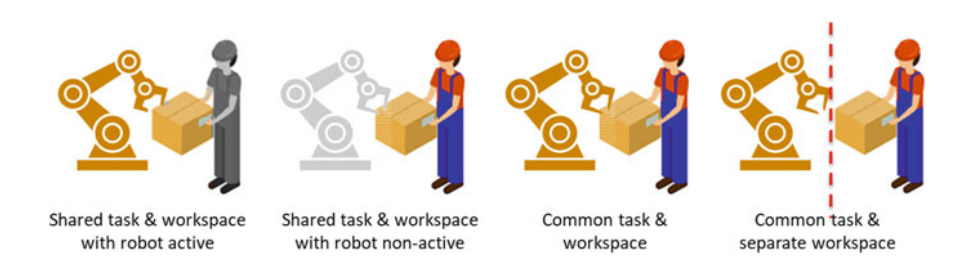
\includegraphics[width=0.8\linewidth]{Figures/Human Robot collaboration.png}
    \caption{Types of Human Robot Collaboration in industrial environment\cite{author3}}
    \label{Fig:1l}
\end{figure}
As the wheel of progress is spinning faster robotics and AI is being advanced in tandem with Big Data, Industry 4.0, and the Internet of Things. The possibilities expanded, expanding far beyond the repetition of modes, technical configurations multiplied, each tailored to the specific demands of tasks, robots, collaboration styles, and production domains.

The integration of collaborative robot systems is a significant leap forward in industrial environments. With careful consideration of the human element, organizations can harness the full potential of this technology, redefining how humans and robots collaborate for increased productivity and safety.

 The International Organization of Standardization (ISO) defines a robot as an “automatically controlled, reprogrammable multipurpose manipulator, programmable in three or more axes, which can be either fixed in place or mobile for use in industrial automation applications” .\cite{author2}
 
 The emerged hybrid production systems aim to alleviate stress and workload blending the strengths of humans and robots. Safety became the cornerstone as robots gained the ability to sense and respond to their environment. Robots can now detect the touch of human hands, adapt to the presence of human workers and even anticipate their motions and conversations by integration of AI in robotics enhancing the safety of Human robot interaction. 
 
 Human-robot interaction is a critical aspect of collaborative robot systems. It encompasses verbal and non-verbal communication, visual information, and gestures, all of which contribute to effective collaboration. In manufacturing, where tasks are often iterative and involve physical interaction, compliance with human states and intent is paramount. While substantial progress has been made in safety within Human robot interaction, challenges remain, particularly in achieving predictability. Designing robots to be tools that humans can understand and control is crucial. This requires formal conditions for system observability and controllability, as well as an understanding of the human's ability to control complex systems.\cite{author3}

While EN ISO 10218 part 1 and 2  were amended in 2011 there were safety measures suggested for human-robot collaboration in the collaborative cell this lead to an exponential rise in the research area of HRC.
Later in ISO/TS 15066, the limiting of forces in different type of robot movement and the design of the robot cells in a safe way were described for collaborative operations of robot with human, but AI integration and introducing cognitive abilities for a collaborative robot is not encompassed in this standards and technical specification.

The research questions we try to address through this thesis are 
What are the potential safety risks associated with AI-Integration in human-robot collaborative environments? How do AI-driven systems interact with other robotic functionalities, and what are the implications for overall system performance? What could be a risk analysis technique for AI-integrated robotic systems? What measures can be taken to ensure seamless integration of AI into lightweight cobots?

We try to answer these questions by studying perception and perception-based application in robotics.
Perception is one technology that is integrated into the robots, which enables the robots to understand their surroundings. Perception allows the robot to identify work material, human co-workers and the dynamic environment in which the robot is. AI-based grasping is one collaborative operation of the robot which can be derived from perception. The robot can grasp an object and pass to humans or humans can work on one object and then the robot picks it up or vice versa.

A process Failure Mode Effective Analysis on AI-based grasping is done in this thesis extending it with System Theory Process Analysis. AI-based grasping algorithms are studied and possible failures of these algorithms are viewed.The Hazard and Risk assessments are based on ISO/TS 12100, keeping in mind the EN ISO 10218-1,2:2011 and the technical specification ISO/TS 15066. 

To increase the reliability of the perception algorithm that induces grasping, different methods are proposed as the result of the thesis. In light of the results from this analysis of risk and hazards a safety framework is formulated for AI-based grasping, which can be taken into consideration, for a generic safety standard for the integration of artificial intelligence in robots.

This is the introduction.

\newpage
\chapter{Literature Review}
% \input{Chapters/Literature_Review}
This is the literature review.

\newpage
\chapter{Methodology}
% \chapter{\section{Methodology}{{\normalfont\fontsize{14}{16}\bfseries}}
This chapter discusses the risk assessment tool used for Artificial intelligence integration in robotics. The tool we use here is Failure Mode Effect Analysis with an extension of System Theory Process Analysis. 
%Since no known standards exist in the market for AI integration in robotics, we use FMEA-STPA as a tool for risk assessment and try to identify the failures and risk related. 
In light of the absence of established standards within the industries and market, we use FMEA-STPA as a tool for conducting risk assessment for the AI integration in robotics, this would help to identify and mitigate the potential failures and associated risks.
The identified potential failures are similar to the data of the Autonomous Driving system. We use FMEA-STPA on perception-based grasping in robots. Since it is one of the best-known scenarios where robots make use of Artificial intelligence and do manipulation tasks. The reason for selecting FMEA and adding an extension of STPA for the risk assessment and the basic definitions of the terms used in processes are explained. The system setup and the boundary conditions are explained in a subsection of the chapter. The use case from which the results are manipulated is also explained along with its relevance.

\subsection{\RaggedRight Robot Bin Picking Application as an Industrial Use Case for the Perception-based Grasping }

In an ideal smart system where robots and humans work together, tasks are split into different jobs, each with smaller tasks. For example, imagine a situation where robots and people team up to pick warehouse parts, put them together a bit, and then move the assembled kits. Some tasks need both humans and robots to work together, while others need each to do their own thing. Besides the main tasks, there are other jobs like fixing problems, figuring out issues, learning new things, giving or getting instructions, handling changes, and planning what to do. Everyone in the system has to work together in these tasks, and sometimes there might be risky situations. %edited by cg

The bin-picking robot system is a highly advanced automation solution designed for the efficient picking and placing of machined parts from two adjacent heavy boxes onto a conveyor belt. This fixed robotic system incorporates cutting-edge technologies, including a magnetic gripper with a spring mechanism that allows robust picking, an RGB-D camera for precise object identification, and Safe Human Detection sensors for human presence detection.

\subsubsection{System Components}

Robot Arm: The robot arm is securely fixed on a stationary base which is a versatile and powerful solution for handling tasks with precision. With a strong payload capacity of 12-14 kg and an extensive reach of 1400 mm, it's well-equipped for various industrial applications. What makes it stand out is its intelligent head, which cleverly integrates Lidar sensors and an RGB-D camera directly into the arm's seventh axis. Unlike traditional setups, this design enhances the arm's flexibility by seamlessly incorporating advanced sensing capabilities. With seven degrees of freedom, it can move precisely in complex tasks, adapting to different orientations. Plus, it's built tough with an IP 65 rating, ensuring resilience against dust and water—perfect for challenging industrial settings. The intelligent head's Lidar sensors enable real-time 3D mapping, helping the arm navigate and plan its path effectively. The integrated RGB-D camera adds high-resolution color imagery and depth perception, making it adept at recognizing objects and handling them precisely. This robotic arm finds applications in manufacturing, assembly lines, logistics, and research and development tasks. Its adaptability, combined with a robust IP 65 rating, makes it a game-changer for organizations seeking advanced automation solutions. Equipped with a magnetic gripper as an end effector for robust and adaptable picking.

Magnetic Gripper: Features a spring mechanism for smooth and secure picking of machined parts.
The magnetic force ensures a strong grip on objects, preventing unintentional drops.

RGB-D Camera: Mounted on the robot arm for comprehensive color (RGB) and depth (D) information.
Utilized for the identification of both the box and the machined parts within it.

Safe Human Detection Sensors: Integrated into the system to identify the presence of humans in the operational vicinity. Provides real-time feedback for safety and operational considerations.

External PLC: The Programmable Logic Controller integrated into the system is used for the human-robot interaction addition to the graphical user interface.

Conveyor Belt: The conveyor belt is placed within reach of the robot arm, to place the object picked from the box. The conveyor belt moves the placed workpiece to the next workstation.

Control System: Manages the overall operation of the robot system and receives input from the RGB-D camera and Safe Human Detection sensors, This System controls the actions of the robot arm, magnetic gripper, and conveyor belt.

The heart of the robotic system lies within a sleek and efficient modular control box. This compact unit seamlessly combines the power of Artificial Intelligence (AI), safety protocols, motion control, and power management. The modular design streamlines the control processes, ensuring a harmonious interaction between these vital components. With AI, the robotic arm gains intelligent decision-making capabilities, adapting to various scenarios. The safety module prioritizes secure operations, and the motion control module enables precise and fluid movements. Simultaneously, the power module efficiently manages energy distribution for a reliable and continuous power supply. This modular control box represents the central intelligence that propels our cutting-edge robotic arm, ensuring optimal performance across a spectrum of applications.

\subsubsection{Operational Sequence}

1. Start-Up: Power on the entire system, including the robot arm, magnetic gripper, RGB-D camera, and Safe Human Detection sensors, Initiate the control system for seamless operation.

2. Picking Phase: The robot arm starts picking machined parts from the first box using the magnetic gripper.

3. Object and Box Identification: The RGB-D camera identifies the box and the machined parts within it with high precision, Safe Human Detection sensors continuously monitor the surroundings for the presence of humans.

4. Orientation Check: The system checks the orientation of the picked object. If incorrect, the robot attempts a re-pick, allowing for up to two failures before corrective actions.

5. Lookup Point and Scene Re-identification: If more than two failures occur, the robot moves to a lookup point.The RGB-D camera re-identifies the box and machined parts, correcting orientation information.

6. Cycle Management: After successfully completing five operational cycles, the system triggers a return to the lookup point.This periodic lookup adapts the system to potential changes in the scene within the box.

7. Human Intervention for Bin Replacement: When the first box is empty, the robot sends a signal for human intervention. A human operator replaces the empty box with a filled one.

8. Placement and Conveyor Belt: The robot continues picking from the second box and places machined parts on a conveyor belt. The robot changes its orientation to keep the time and avoid singularity errors during pick and place from the second box.

9. Specific Placement: The robot is programmed to place objects precisely in a predefined location. The magnetic gripper ensures a controlled release, preventing unintended drops.

10. End of Cycle:The operational cycle completes within the designated 28-second timeframe.

\begin{figure}
    \centering
    \begin{minipage}{0.8\linewidth}
    \centering
        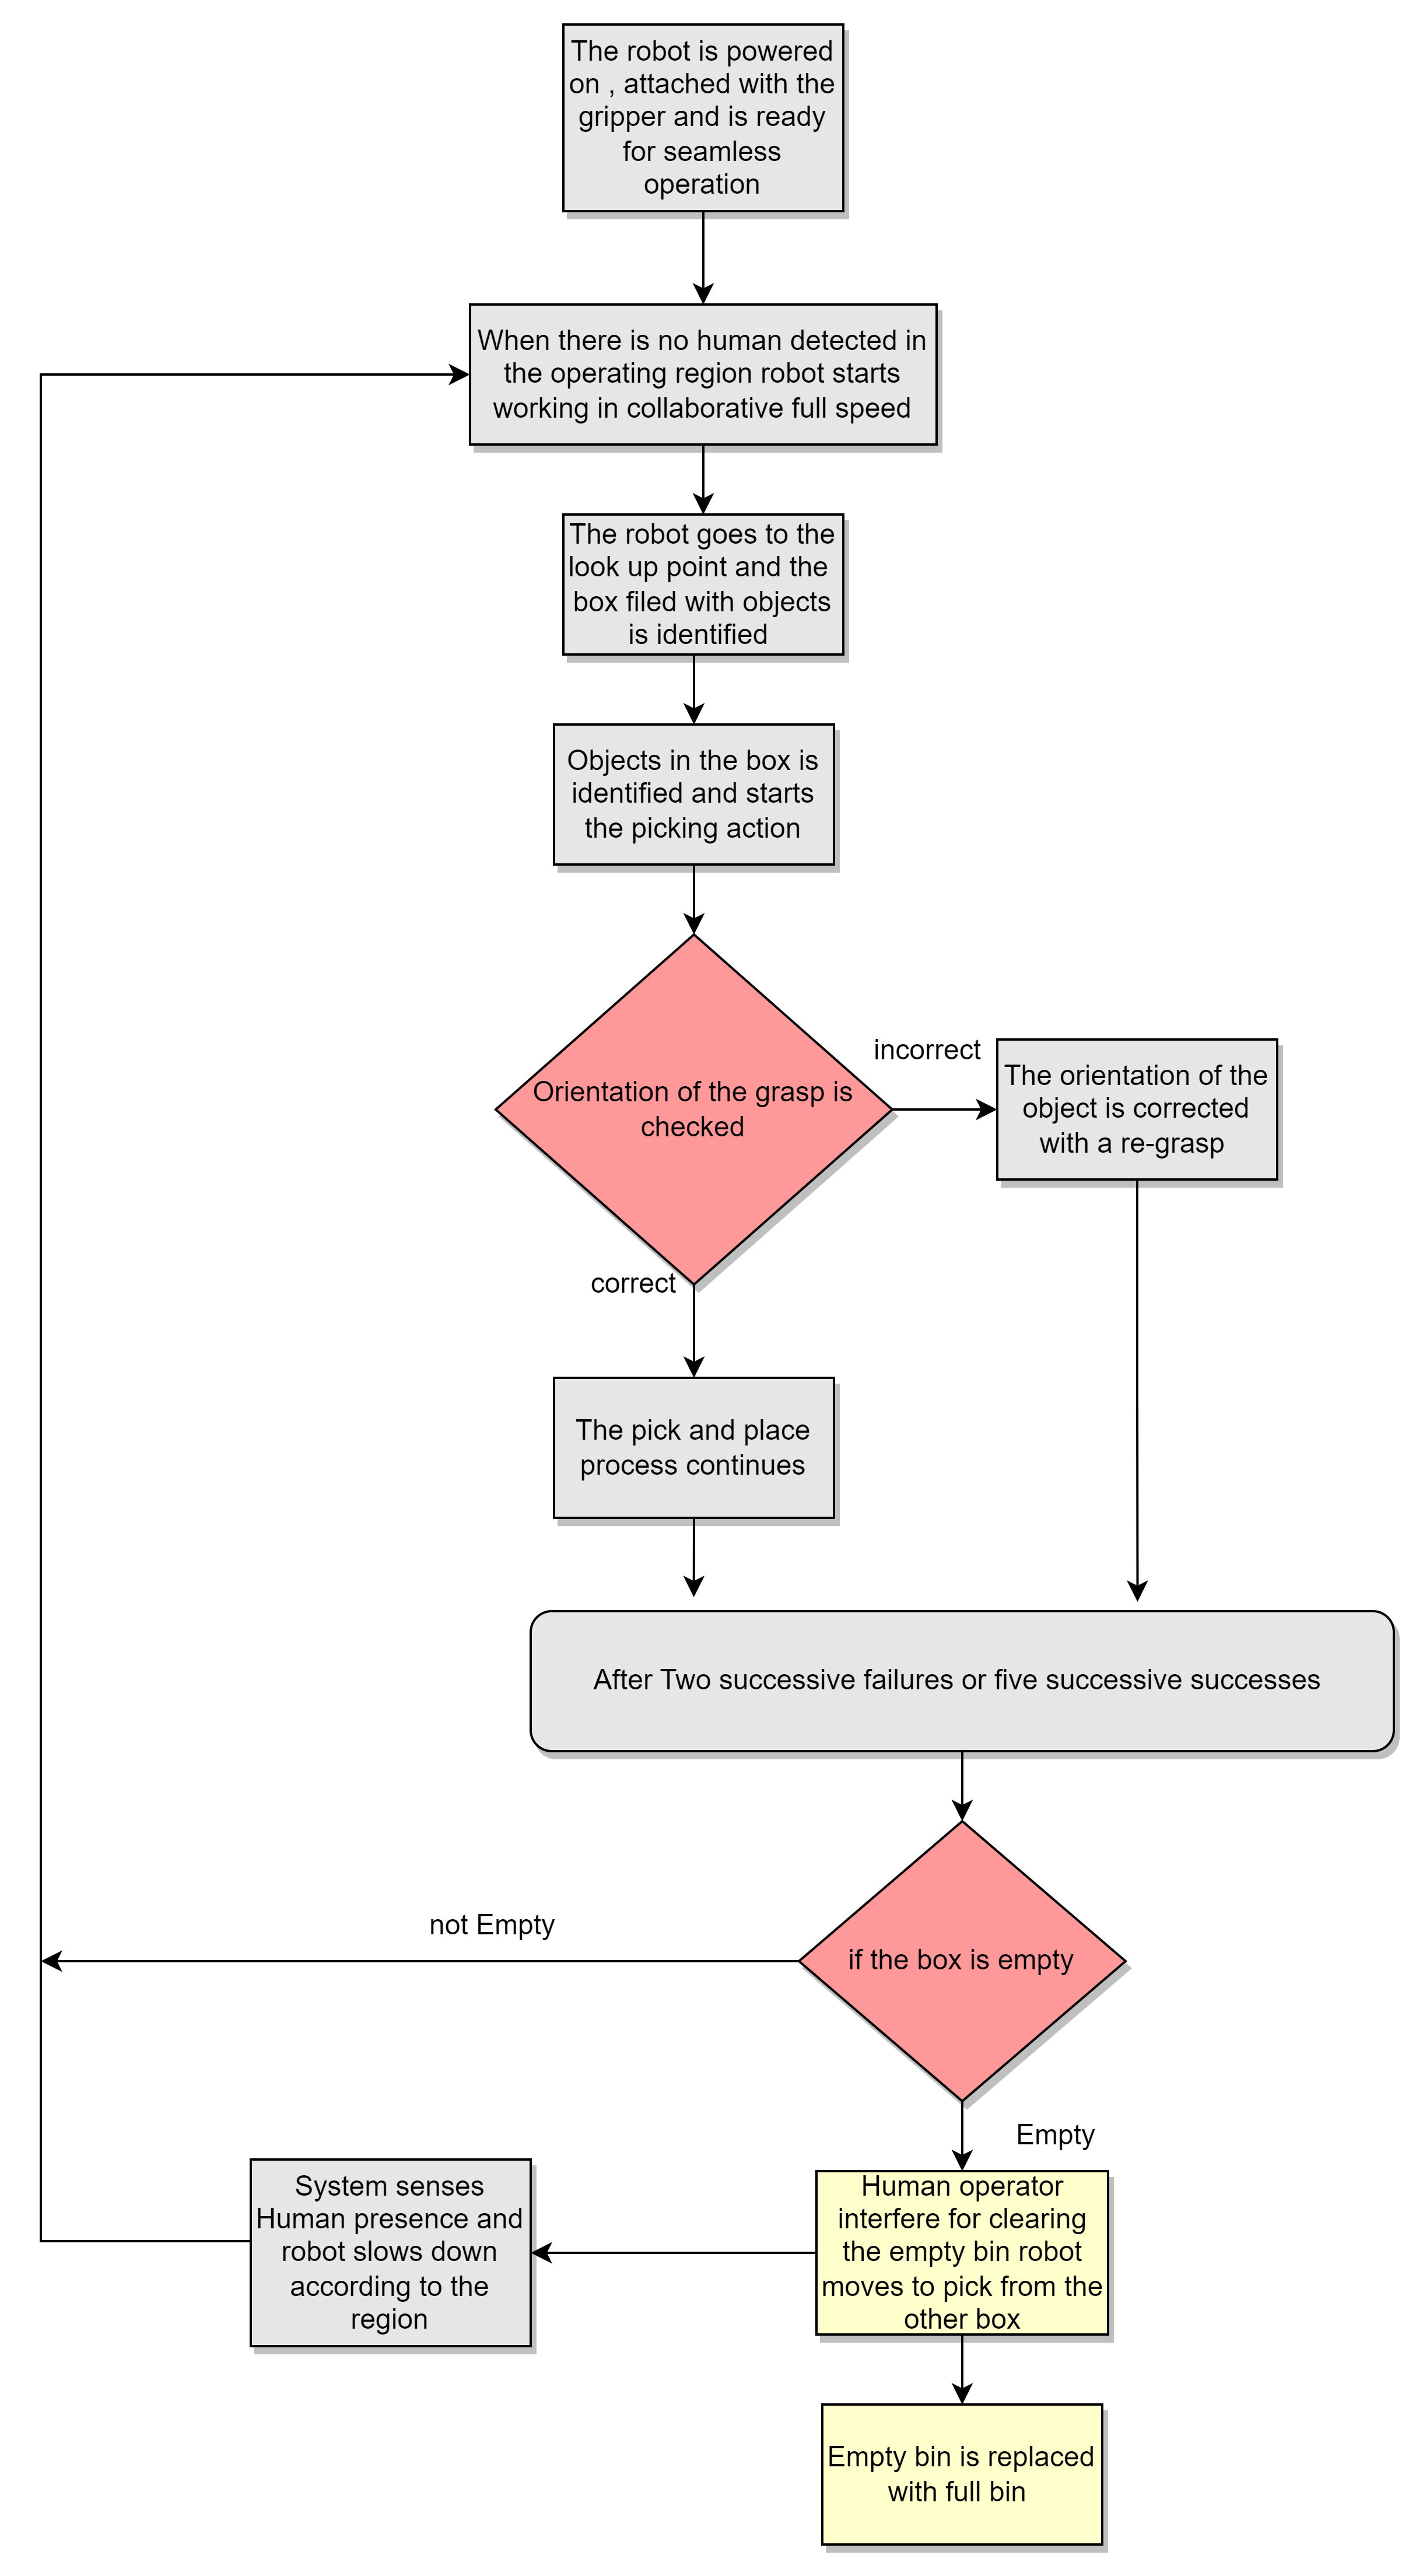
\includegraphics[width=0.5\linewidth]{Figures/SOP_flowchart.png}
    \end{minipage}
    \label{fig:enter-label}
    \caption{Flow chart of the Standard Operating Procedure}
\end{figure}

The bin-picking robot system integrates state-of-the-art components to deliver a reliable and precise solution for the automated handling of machined parts. The combination of a magnetic gripper, RGB-D camera, and Safe Human Detection sensors ensures efficiency, safety, and adaptability. The system's ability to manage potential failures and periodic lookups contributes to its overall robustness and reliability in a manufacturing environment. Regular maintenance and adherence to safety protocols are crucial for optimal performance.

 \subsubsection{Control Structure}

In this system, there are two computers, one would be processing the AI inputs and then sending signals to the other computer which would control the robot with the software. The AI computer after recognizing the object would send the coordinates of the detected object to the control computer. The calculation of the forward and inverse kinematics is done inside the second computer in this case, and the optimal way of approaching the workpiece is found out using this.
The AI computer also sends information about the force to be used by the end effector to pick the object according to the object identified. The Robot-Human interface allows feedback from the operator as well as helps the robot to send signals about its actions.
The number of successful picks and the successful failures are being monitored for this particular application to trigger the movement of the robot to look up point.

The orientation of the pick is monitored, if the orientation is not as expected, then the robot puts back the workpiece. If there are two failures in pick, and then the robot puts back the workpiece the robot has to go to the look up point , There are control triggers from the AI system in these two scenarios

The control unit would have the state and orientation of the robot which is being updated in every one millisecond by the heartbeat signals.
There are passive safety controls like collision detection and safe torque ON when the robot detects anomalies in the voltage behavior and the external forces.
The Safe Human Detection sensor senses the human or any obstacle inside its perimeter and then the robot slows down or the robot stops according to the region where the human is detected the Safe Human Detection sensor is connected to the Digital input of the system. 
As soon as there is an obstacle in the region the Safe Human Detection sensor sends the signal high into the Digital inputs and then the processor first assesses the state of the robot and then asks the robot to slow down or to stop or to be in stop mode according to the state of the robot. 
The monitoring of the robot limits cartesian space and the joint space is continuously happening. This is also limited according to the present ISO standards and technical specifications for the safe operation and integration of robots.





%The limits of the robot are set optimally for the three cartesian coordinates and the orientation of the tool center point to the base and joint space are limited for safety purposes, thus unexpected rotation of the robot arm will not happen, even when the robot is in hand guiding mode.



 \begin{figure}
     \centering
    \begin{minipage}{1.0\linewidth}
     \centering
        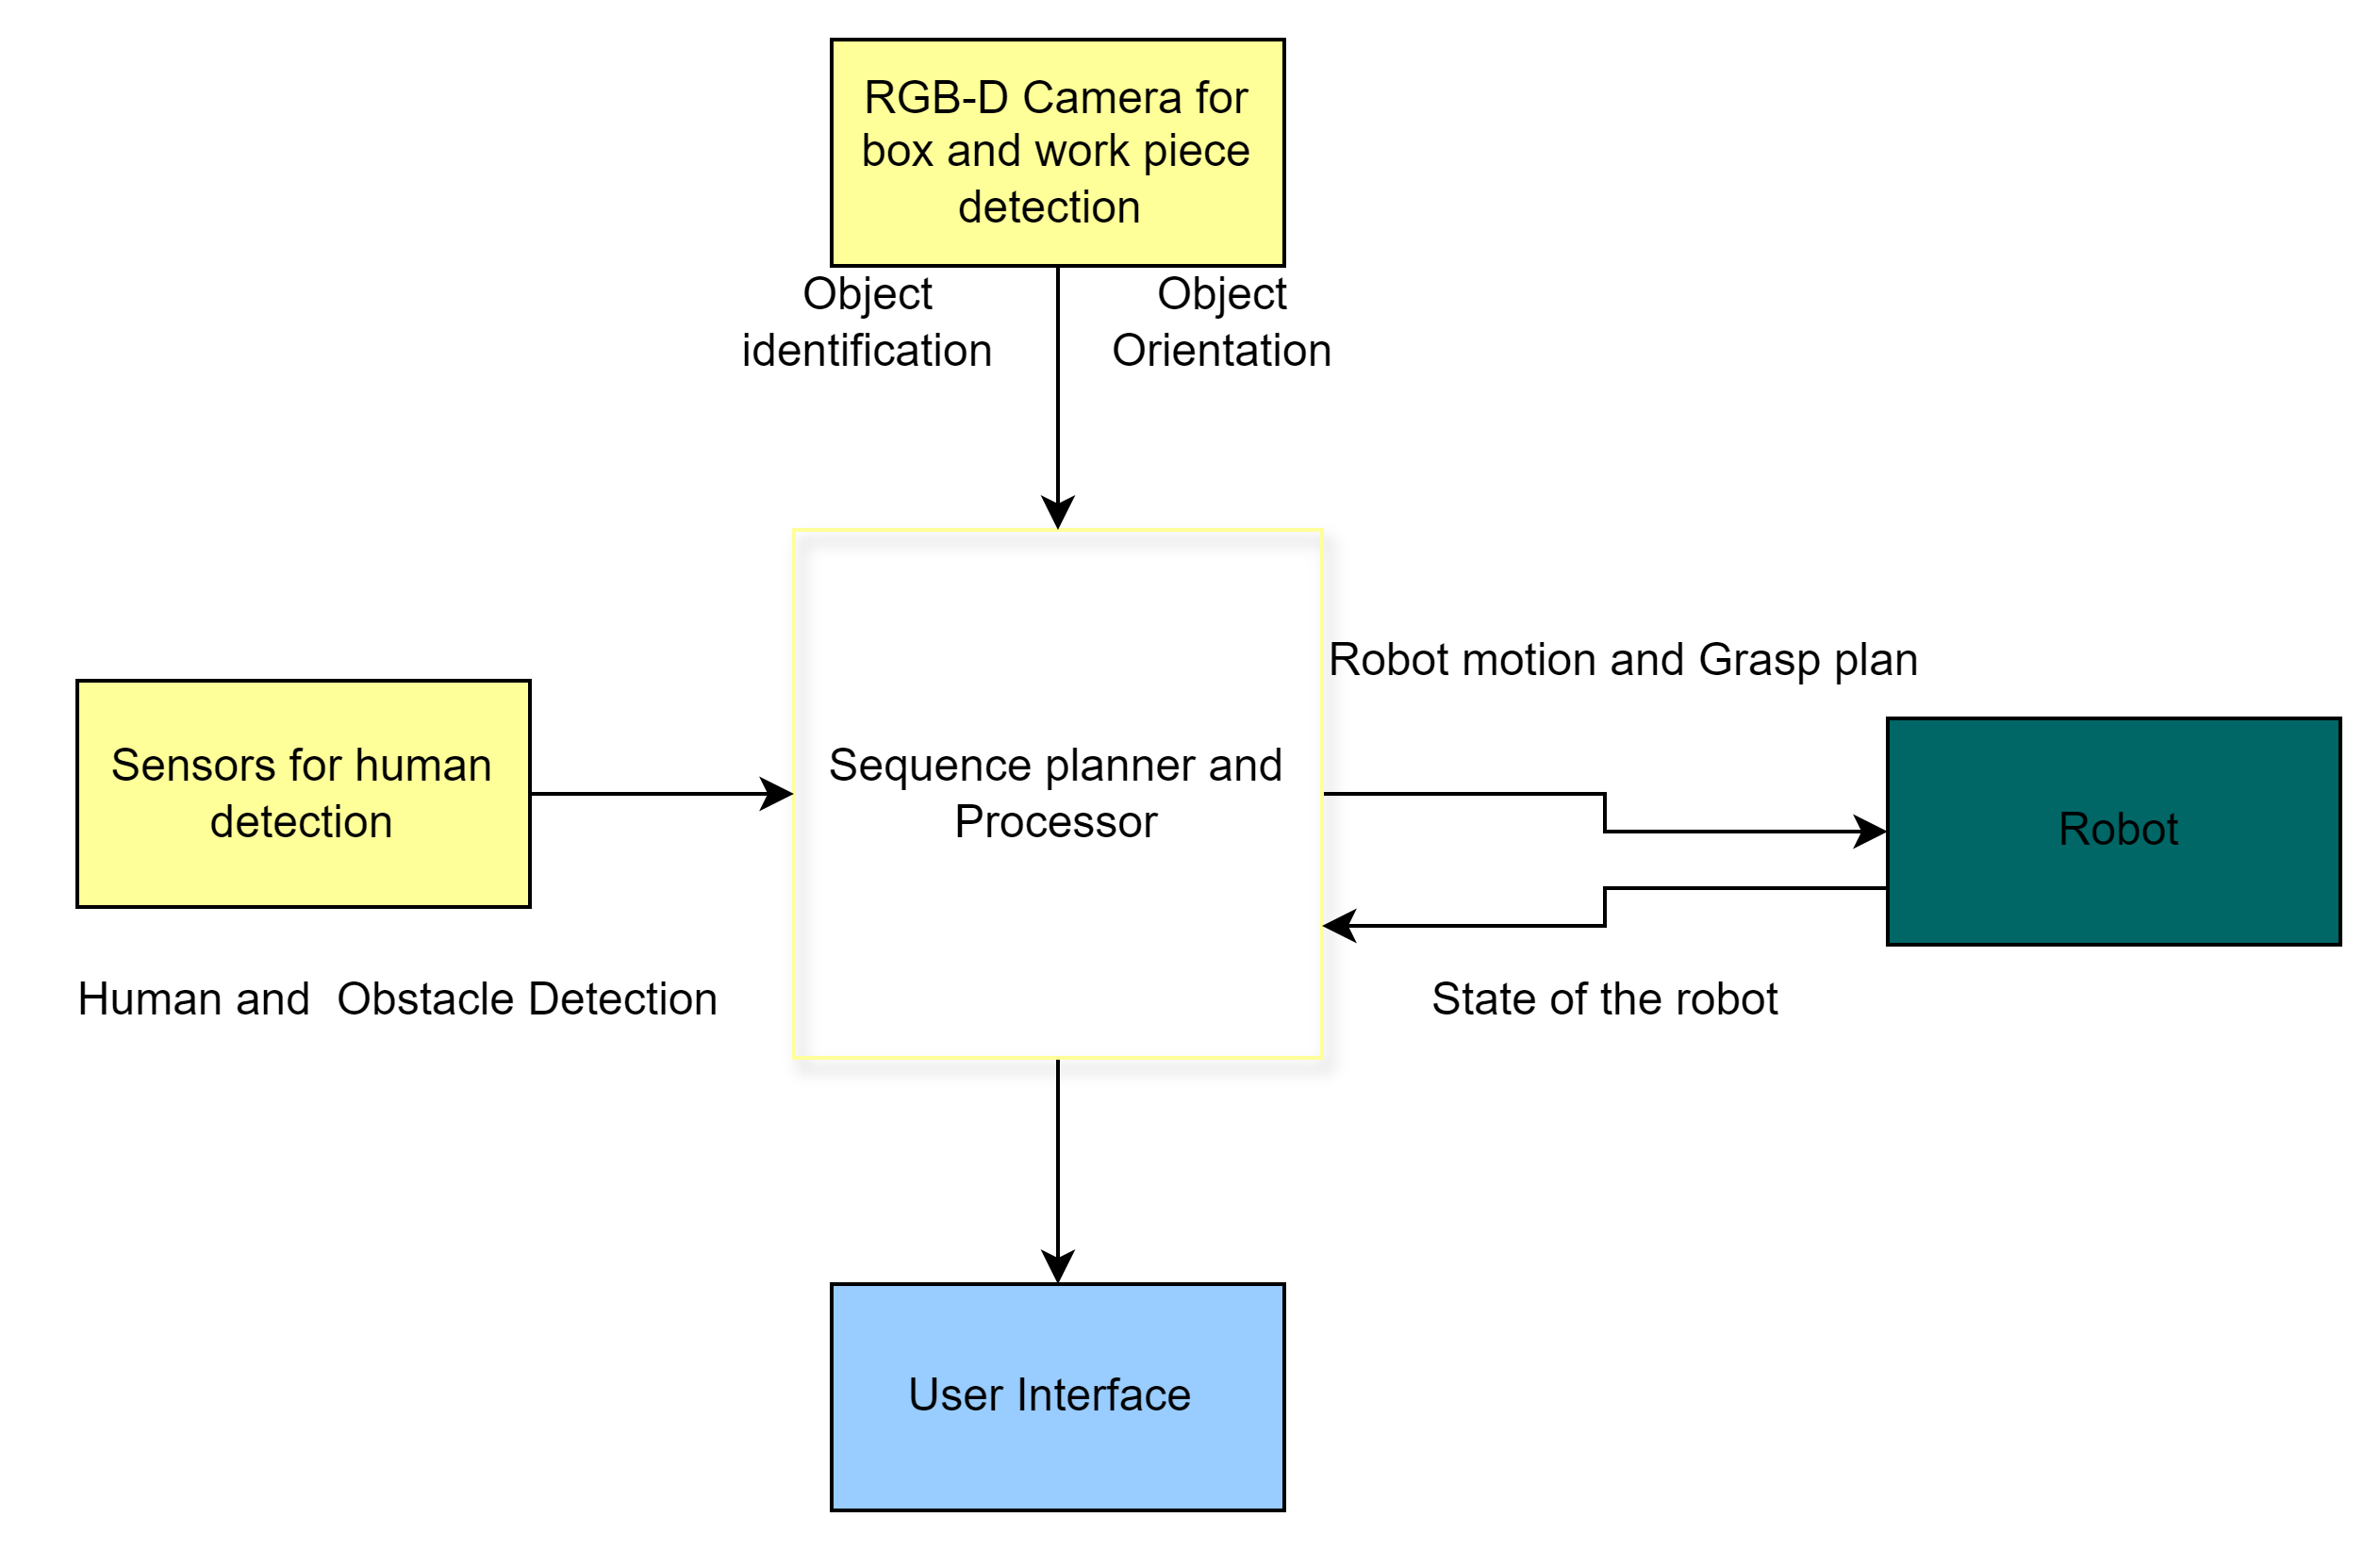
\includegraphics[width=0.75\linewidth]{Figures/Control_Structure.png}
        \centering
     \caption{Control Sequence:Inputs from sensors,processing and output}
     \end{minipage}
     \label{fig:enter-label}
 \end{figure}
 

\subsection{\RaggedRight Risk Assessment Methods and Tools }

 The ISO/TS 15066 or EN ISO10218-1:2011 and ISO 10218-2:2011 do not specifically  dictate a special risk assessment method. ISO 12100:2010 suggests a task-based risk assessment methodology to determine the performance level required for the safety functions.
 
 To enhance the system and process safety there are many techniques available such as FTA, ETA, HAZOP, FMEA STPA, etc. 

Fault Tree Analysis (FTA) is a top-down risk analysis method that examines an entire system by breaking it down to components and analyzing the conditions that may lead to a predefined problem. This problem is called the top event. Defining the top event, decomposing the system into individual components. Identification of relevant events and conditions, and establishing the logical relationship are the main steps of FTA. FTA allows quantitative and qualitative analysis. The result of the analysis is documented using the Fault Tree diagram, illustrating the logical relationship and the need for improvements in the system safety measures.

Hazard and Operability Studies (HAZOP Studies) are a risk analysis technique for a defined system, identifying potential risk in operating and maintaining the system and external risk sources like environmental hazards that can trigger risk for the system itself.

Then we have risk assessment techniques like Failure mode effects (FMEA) which break down the system and analyze the risk of each of the components or each step of the process. 

System Theory Process Analysis (STPA) is a comparatively new risk assessment tool that can be used to study the control structure of the system, how the interactions between the components are processed, and analyze if there are unsafe control actions.

FMEA and STPA are discussed further in the next subsections as we are doing our risk analysis of the AI-integrated robotics system using an extension of FMEA with STPA




\subsubsection{\RaggedRight Failure Mode Effects Analysis }
FMEA is an engineering analysis method to be used to analyze the system from bottom to up for the design of new systems, 
 new processes, new software, and later to improve production and design. It is useful to evaluate failures that may occur, the effect of the failures on the system, and mitigation strategies. EN IEC 60812:2018 is a standard that specifies how to use this risk assessment tool effectively in the industry. This standard illustrates use of FMEA in different scenarios. 

FMEA applies to hardware, software, and human action interface between humans and hardware or software in any combination. This could be used in any stage of the lifecycle of a product, process, or system. It is based on the reliability theory.

The four stages of FMEA are preparation, risk identification, risk assessment, and risk reduction. The preparation stage is where the boundary conditions are explained the process flow chart is drawn and most importantly the decisions about what should be included and excluded are considered. Risk identification starts by identifying and describing the function of relevant steps in the process and each item's potential failure modes. Risk assessment could be done by finding the RPN and estimating the likelihood of failure. Risk reduction is the step where corrective actions are developed and implemented.[30]

The analysis starts from the lowest component and proceeds up to the failure effect of the overall system. A failure effect of a lower component can be a failure mode for a component at a higher level. The potential problems in the design and development of the system can be studied.

There are different applications for the FMEA considered such as the software FMEA and the process FMEA. The software FMEA can be used on embedded real-time systems. Software FMEA is a very important failure analysis method since the software does not fail randomly and all the software failures are systematic failures, due to wrong specifications or requirements of the function.

In this analysis, each failure mode portrays the potential failure of the product or system and these failure modes' cause of the failure and the effect of the failure are entered in the spreadsheet called the FMEA table. 

In this research, we use process FMEA to analyze the process, where the robot is used to pick and place the workpiece using integrated artificial intelligence. We break down the process into steps and substeps and do the analysis 
 
 The integration of Artificial intelligence in robotics introduces a paradigm shift that brings several risks into the scenario. We use FMEA as our risk assessment tool and not other tools like HAZOP, Fault Tree Analysis, Event Tree Analysis, or Common Cause Failure Analysis because of its unique features.
  
  FMEA is useful in identifying causal factors such as interface errors, Hardware and software interaction, and software defects in the usage of improper protocols or even the architectural mistakes in the software of the system.
 
 FMEA allows the breakdown of the system into constituent parts so that the identification of risks is possible at the component level. In the context of AI in robotics, it is essential to break the system into constituent parts as there are many intricate algorithms and dynamic decision-making processes in the control system.
 
 The proactive nature of FMEA also was a reason for us to choose this risk assessment tool. The other risk assessment tools use the reactive method after the occurrence of the risk. This is suitable for dynamic environments and real-time decision-making.

FMEA allows quantitative and qualitative analysis of risk. The severity, occurrence, and detection of the failure modes contribute to the quantitative analysis of the risk while the team's expertise and experience could add qualitative insights. 

FMEA allows cross-disciplinary collaboration, experts from robotics, Artificial Intelligence experts, other engineers, and domain specialists. This allows views from different angles to a problem and could lead to more robust risk reduction. The algorithmic biases uncertainties in learning and adaptability to complex situations can be tailored using FMEA. 

FMEA encourages the thorough documentation of the risk assessment processes. The documentation is invaluable to trace back the actions taken. This documentation is also essential for the certification processes. In the rapidly growing field of AI, having a well-documented risk assessment methodology is essential for presenting in due diligence of the AI-based control systems.

FMEA deals with the known potential failures and introduces new countermeasures to mitigate the negative effects., it is hard to identify all risks in the early phase of the development using FMEA. Especially for intelligent control systems that may make their own decisions.



\subsubsection{\RaggedRight System Theoretic Process Analysis }

System Theoretic Process Analysis-(STPA) is a top-down proactive method for analysis that is based on the System Theoretic Accident Model and processes. This is a relatively new method of risk analysis that is beyond directly related to failure events or component failures but to more complex processes and unsafe interactions among system components.This analysis is mentioned in ISO 21448:2022 which addresses functional insufficiencies of systems.

STPA uses a model of the system that consist of a functional diagram of the control system not really the physical parts in the control system but how the interactions are being worked.

STPA also includes Planning, which means defining the purpose of the analysis including the definition of the system, and boundary conditions. Identifying system losses and hazards. The second step is creating a hierarchical diagram of the control structure. The third step in STPA is an analysis of the control actions. The next step includes describing the causal factors that can include unsafe control actions and hazards, translating uncontrolled actions into constraints on the behavior of each controller. The unique features of STPA enable the risk assessment of the control systems.

STPA defines hazard as the state of a system or condition that could lead to an accident. Since an inadequate control action can lead system to a hazardous state . STPA studies whether a control action required is provided, if the control action provided is safe if the control action being provided in wrong time or sequence and if it is provided in inadequate timing.

In this study of the control actions we consider communication failure for example delayed failure or corrupted communication inside the system since the delivery of the control command to the component from the processor is also an important aspect of this.



The systemic approach in which the whole system is considered and the interaction between the components is analyzed rather than doing risk analysis on individual components. It helps in the holistic concept of the system and the potential vulnerabilities of the system.

STPA analyses the processes inside a system. The hazards arise from interactions of the components inside the system which allows a nuanced understanding of the system working.

The proactive approach of STPA allows the early detection and identification of potential hazards, which allows for the prevention of the hazard being embedded in the system in the development cycle itself.

The strong emphasis placed on control systems by STPA examines the working of the control system and identifies the deviation from the correct working of the system. This in turn helps in identifying enhancements in control measures.

STPA not only considers technical aspects but also takes into consideration the human factors and organizational factors that could cause hazards. This helps in a holistic approach to risk assessment which could include technical and human-related risk.


The causal analysis method employed by STPA allows to identification of root causes for the potential hazard which could help in more effective mitigation of the risk from various factors contributing to the risk.

STPA is being adapted in different fields like the automotive and aerospace industries for risk assessment in intelligent control systems. This could also be used in the field of robotics.

STPA considers hazards as a challenge in managing system controls, encompassing not just failures but also hazardous successes. This implies that even if individual components operate successfully, their combination may still result in a loss of system integrity. As a result, STPA is frequently utilized in safety-critical systems and scenarios where the most severe outcomes need to be anticipated.

A notable limitation of STPA in risk assessment is that we cannot quantify risk using STPA for example there could not be an RPN number if we use STPA for risk analysis.

\subsubsection{\RaggedRight Risk Assessment using FMEA-STPA } 

The purpose of this project is to conduct risk assessment for the perception-based grasping system in robotics. The analysis aims to identify, evaluate, and address potential failure modes in the perception components, algorithms, and related processes to enhance the safety, reliability, and performance of the grasping system. This may include Assessing the Sensors, Object Recognition Algorithms, Environmental conditions, Integration with the Grasping mechanism, Communication, and Data processing and how this might affect human-robot interaction.

For risk assessment of the AI systems in robots, we use the tool FMEA with an extension of STPA, which is strongly advocated by the authors of \cite{author30}. To overcome the limitations of both the tools we use this extension. We use a brainstorming session for the effect cause analysis of the identified potential use case.

For FMEA which is a bottom-to-up risk assessment strategy we study each component in the process and for STPA which is a top-to-down risk analysis we study every interaction of the components in the system and the risk assessment according to the recommendation of the standard EN ISO 10218-2:2011 for robotics systems which suggests a structured risk assessment. Since it is difficult to find out the occurrence and detection of intelligent systems we use STPA for the controllability of occurrence and detection using.

The tool complements the shortcomings of each other. For example, FMEA is component-centric or event-focused, this can lead to dangerous success meaning even if the components are not failing the whole system working together can cause a failure leading to a hazardous event. this can be monitored using STPA which identifies the risk at the system level or according to the process.

While FMEA gives the prioritized actions for the mitigation of risks. STPA gives safety requirements to be followed based on technical and human aspects of the system. The integration of these tools could be a better way to assess the intelligent complex systems

The process requires a well-experienced system engineer, robotics engineer, AI specialist, a Product manager who decides the requirement for the system, and A Functional Safety expert as the first step of the risk assessment.


We try to quantify the severity, occurrence, and detectability on a scale of 1 to 5. We use the STPA and the definition of the control structure for identifying unsafe control actions.
It is crucial to tackle a particular type of risk arising from uncertainty, as responses or inputs/feedback can be appropriately supplied at the right moment (neither prematurely nor belatedly). The combination of these methodologies the advantage is FMEA gives the potential risk of failures in process aspects and the STPA gives the potentially unsafe control actions that could influence the acting decision of the system. 
Thus when we quantify risk , we think the logic, if there are control actions for a particular error arising due to malfunction of the components, the occurrence rating would be less for this error, which can lead to a failure, Similarly if there is no control for a particular failure, the occurrence rating would be very high. This is similar in case of detectability also. Thus STPA is relevant in the risk assessment of the intelligent control system which give inputs for the robot actions.

 However, this entails inherent uncertainty, especially when utilizing machine learning techniques. For example, when the vision system furnishes information to the control system regarding the operator's position, the algorithm may exhibit uncertainty regarding the precise position, particularly if the human is partially obstructed. This uncertainty will place restrictions on when the control system can carry out an operation. In the brainstorming session, these failures arose from uncertainties that were considered, and the possible remedies were discussed. 
 

\vspace{0.5cm}
\subsubsubsection{ \textbf{Failure Modes}}
\vspace{0.2cm}

When we do the Failure modes effect analysis for the process each step of the process is considered and the failure modes are determined. Each step of the process is then subdivided and failures are determined.

\begin{figure}
    \centering
    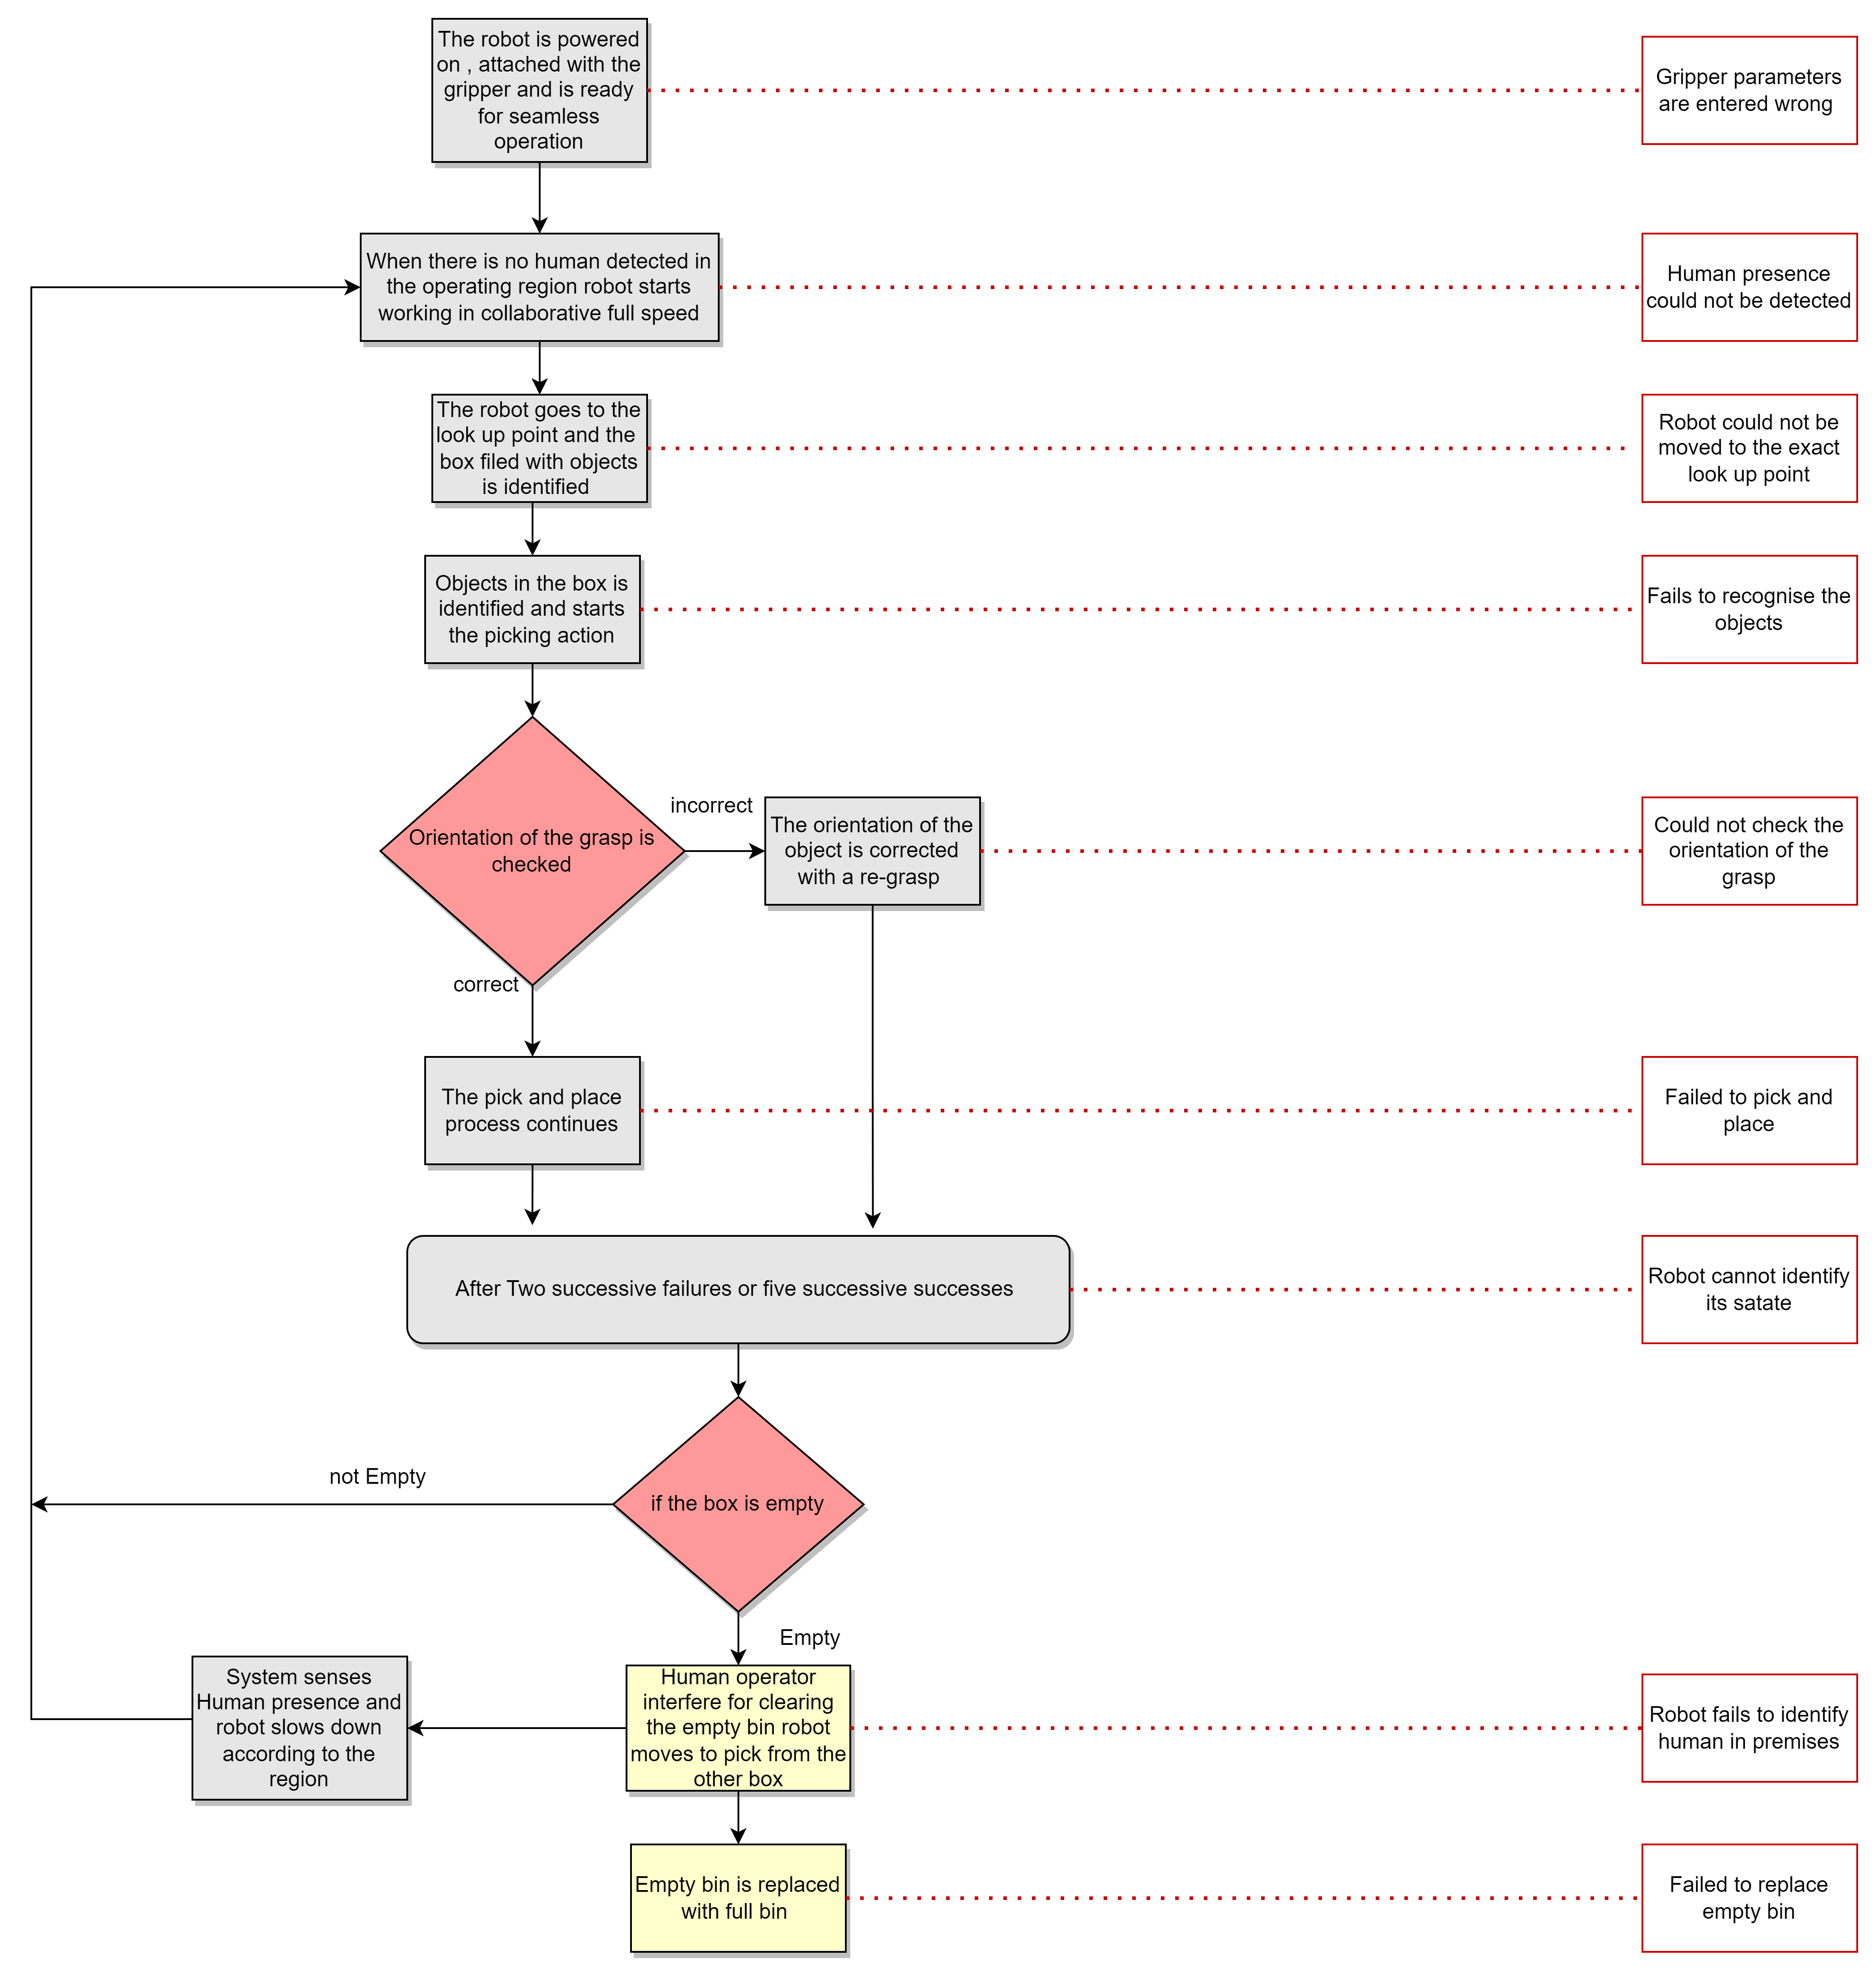
\includegraphics[width=1.0\linewidth]{Figures/Failure.png}
    \caption{Failures Identified in Standard Operating Procedure}
    \label{fig:enter-label}
\end{figure}

So when we consider the industrial use case for grasping it can be divided int 4 major phases which can be subdivided into steps for the FMEA, which are Object Identification Phase, the Picking Phase, the Placing Phase and the Human intervention phase.

We can divide the  Object identification phase into substeps like Object detection, Object identification, and Grasp Estimation.
The following failure modes could arise in the above phases.

1. False positives: The system detects objects even if the bin is empty.

2. False Negatives:  The system is unable to detect objects inside the bin even if there are objects inside the bin.

3. Over-segmentation: Here the system takes the input and can see one object as two or more due to over-segmentation.

4. Under-segmentation: Here the system takes the camera or sensor input and sees two or more objects as one due to under-segmentation.

5. Occlusion: The system is unable to recognize the objects that are occluded due to the objects above in the box.

6. Incorrect Identification of Object: The system could incorrectly identify the objects and may damage the object due to this.

7. Incorrect Orientation Recognition of Object: The system incorrectly recognizes the object's orientation.


The second phase can be divided into substeps where the robot moves to pick the object, the robot applies the correct force to pick the object and then finally grasps. In this phase after grasping the robot checks the orientation of the object after grasp.
The following failure modes could arise in the above phases.

1. Incorrect Orientation of the Gripper to Pick the Object: The gripper is oriented incorrectly, which could cause the pick of the object incorrectly.

2. Incorrect force for pick.

In the 3rd phase, the robot places the object and this can be subdivided into the moving phase where the robot holds the object and moves to the final destination, and the placing phase in which the robot places the object in the required orientation.
The following failure modes could arise in the above phases.

1. Objects could be misplaced on the conveyor belt could cause damages

2. Misalignment of the robot arm during the process




Human intervention is asked, whenever the box is empty for replacement. In the Human intervention phase for replacing the bin the following failures could happen, the Safe Human Detection sensor is used for detecting human approaching and the outputs would be different as there are zones for the human to interact with the robot.
The following failure modes could arise in the above phases.

1. False negative in human identification: The system fails to identify the human presence near the system

2. Human Location Uncertainty due to Occlusion: The system identifies to detects human presence but cannot identify the exact location of the human due to Occlusion

3. Delayed Human Detection: This can cause great danger for the operator, this is a severe failure mode where there is a delay in human detection due to communication breakdown between sensors and processors or high computing time for the processor. 

\vspace{0.2cm}
\subsubsubsection{ \textbf{Control Analysis}}
\vspace{0.2cm}

%In addition to problems caused by the failure of specific functions or components, interactions or control problems between system components are considered as hazards, and are effective in identifying the hazards based on unsafe control actions between components


We do a Control Analysis, to understand the communication control actions and the feedback loops between the AI system and the robot control system. The first phase of the analysis is the assessment of the clarity, reliability, and efficiency of data exchange.

The analysis also includes whether there are control actions provided, not provided or provided with timing discrepancies. This assessment may help to find out the vulnerabilities of the control mechanism. The timing discrepancies mean if the control action lasts too long, if the control action stops prematurely if it happens too early, or if it happens too late.

One of the major control actions in this use case is the robot reducing its speed as soon as the system detects a human in the virtual cell where the robot is working and, when the human operator is in the second region inside the collaborative workspace that is very close to the robot, the robot stops all its movements. This action starts at the moment the human steps inside the region and lasts long till the human is moved out from this region. This is one of the active control mechanisms which is used to avoid collision between the operator and the robot.
Detection, Evaluation and Identification of the box and the objects are control actions which is provided just before the pick is started 

The trigger to pick and place the object. The other control action is providing the required force for holding the workpiece by the magnetic gripper. As soon as the object is identified and the robot is near the object for pick. the magnetic force should be provided for the pick. This would last till the object is placed in the correct place.

Changing the states of the robot and the whole system is an action provided by the control systems from its inputs.  When analyzing the system's change of state for some of the potential failure modes we found that, there is a lack of control action thus limiting the dangerous success of the robot operation. Thus few of the control actions are recommended to be implemented for the perception-based pick-and-place robotic system.

These are the implementation of fail-safe mechanisms and predictive maintenance and analysis of the sensors on the robot and the sensors in the surroundings. This is discussed in detail in the next chapter. The need for planned safety also arose from this control analysis a small description for the need for planned safety is described.

In short, this control analysis also helps to analyze the interactions between the components, which helps in finding not only the failure of specific components or function of the robot but the unsafe control actions too.

\vspace{0.5cm}
\subsubsubsection {\textbf{Uncertain Failures}}

The uncertain input controls from the vision system and the sensors on the robot and the application environment reduce the trust in the system. This also acts as a barrier for the system to reach the required performance level with safety. 

The uncertainty in the position of humans or any obstacle in the robot's path or in the surroundings should be reduced. The uncertain events and the events with no control preventions are identified with this process.

To implement the planned safety, this is important. An approach of planned safety and active safety together is essential for the robot system integrated with AI to mitigate unknown risks thus a deliberative safety implementation is used by the control software of the system thus the unintended signals would not be produced by the control system.  Planned safety is an approach defined by the researchers [35] for integrating intelligent human-robot collaboration in Industry 4.0. This approach helps in rectifying the uncertainty from the vision system and other sensors used in the system.

%We found the major failures for the use case after compiling all the steps involved in the process and then breaking down the process according to the SOP. as Sensor Malfunction, Object Recognition Errors, Communication Breakdown, Environmental Changes, Algorithmic Errors,	Human Interference, Calibration Issues, and Safety Violations.



%The Effect-Cause Analysis is done for the identified failures also done in the brainstorming session



 
\subsubsection{\RaggedRight Decision Criteria for Treatment of the failure modes }

The Decision criteria for the treatment of the failure modes are based on various factors such as the severity, controllability, and probability of detection other factors like complexity integration of the treatment action to the system and the effect on the performance matrix are also considered in the decision criteria. The risk matrix is found  out of the severity, occurrence, and detectability found in the table.

Here severity is assessed by taking the potential failure effect into account. We use a five-point scale for this. The reasons and the failure mechanism is also noted down in while severity is being checked

\begin{table}[ht]
\centering\
\begin{tabularx}{\linewidth}{|X||X||X|}
\hline
 Rating & Description & Criteria \\
\hline
1 & Very Low &  Objects not picked correctly \\
\hline
2 & Low & compromise in cycle times, Objects not placed correctly \\
\hline
3 & Moderate & Robot colliding, damage to the workpiece, damage to the obstacle\\
 \hline
4 & High &  Damage to the robot, System shutdown\\
\hline
5 & Very High & Injured Operator, Fatality\\
\hline

 \end{tabularx}
  \caption{Severity Rating (S) Table}
\end{table}

While analyzing the probability of the occurrence and detection the usage of the STPA comes into the scenario where we analyse whether there are control actions provided for this potential failure mode, if the control action is provided if it is sufficient, and if it is efficient. 
    
The probability of occurrence is taken into account considering the system's complexity, potential failure mode, and cause of failure which is also in a five-point scale. The uncertain control actions are also mentioned in this part of the table. If there are no control actions provided for this from the system the maximum occurrence rating would be assigned for this cause of failure mode.

Thus instead of quantifying the failure rate we consider whether the control action provides prevention from the failure and based on the provision of the control action and based on the efficiency of the control action we try to number the control prevention. If there is suitable control prevention to protect against potential failures, then it is given 1 and if there is no control prevention at all then it is numbered 5. The occurrence rating  from 2 to 4 is assigned based on the suitability and length of the control action provided.


\begin{table}[ht]
\centering\
\begin{tabularx}{\linewidth}{|X||X|}
\hline
 Rating & Criteria \\
\hline
1 & Suitable and Efficient Control Provided \\
\hline
2 &  Suitable Control prevention for prolonged time   \\
\hline
3  & Suitable Control Prevention but wrong timing (too early or too late) \\
 \hline
4  &  Suitable Control Prevention but  for short time \\
\hline
5  & No Control Prevention \\
\hline

 \end{tabularx}
  \caption{Probability of Occurrence Rating (Po) Table}
\end{table}

Detectability is assessed on a five-point scale based on the complexity of the component and the potential cause of failure. The detectability is also measured by the ability of the processing unit to detect whether there are potential failures for the intended functionality.

If there is no detection of the cause of failure then the probability of detection value would be considered the highest. If there is suitable detection for the cause of failure then it would have the lowest rating. 

\begin{table}[ht]
\centering\
\begin{tabularx}{\linewidth}{|X||X||X|}
\hline
 Rating & Description & Criteria \\
\hline
1 & Almost Certain Detection & Detectable at least 90 percent of the time of failure \\
\hline
2 & Highly likelihood of detection &   Detectable at 75 percent of the times of failure\\
\hline
3 & Moderate &  Detectable at 50 percent of the times of failure \\
 \hline
4 & Low likelihood of detection & Detectable at 25 percent of the times of failure  \\
\hline
5 & No Detection & Detectable at less than 10 percent of the times of failure \\
\hline

\end{tabularx}
  
\caption{Probability of Detection Rating (Pd) Table}

\end{table}


Later the Risk Priority number (RPN) number is calculated by multiplying the Severity value by the Probability of occurrence times the Probability of Detection.

According to the RPN obtained for the failure modes we prioritize the mitigation methods to reduce the risks with the highest RPN. The categorisation of the RPN is explained in the next section
The mitigating actions proposed should bring the risks to an acceptable level. Active safety and planned safety approaches can be used to bring down the risk to a minimum.

After the reduction of the risk, the process can be iterated to identify new potential failures and risk reduction methods. The SOP should be altered in such a way that these process failures are mitigated if needed or the system requirements should be changed in order to reduce the RPN thus the detectability and the controllability of the very severe risks can be brought down.

The major results of the risk analysis were the implementation of the control actions for the potential failure modes, including upgrades in the sensors used, and the introduction of predictive analysis algorithms for the sensors, thus detecting anomalies in the sensor behavior. This is explained in the next chapter.




% 1. Partition the system to be examined into subsystems and components, taking the
%architecture of hardware and software into account.
%2. Assign the application function to each component. In this step, functional and nonfunctional requirements have to be interpreted.
%3. Determine and analyze the potential failure mode, cause of failure, and failure effect
%that can lead to a hazardous state. For instance, the failure mode “false break activation”
%could have the cause of a defect in the SW of pressure determination and the effect
%of a potential crash situation between two cars. Another example regarding security
%is, for instance, a failure or threat mode classifying the way in which vulnerabilities
%are exploited (Schmittner et al. 2014). A threat mode could be “attacker is pretending
%to be a measurement device” violating the integrity of the system. The cause could
%be an encryption problem or security breach and results in “system is unreliable and
%potentially unsafe.”
%Each failure mode represents potential product failures that can occur. Failure mode,
%cause, and effect are entered in the spreadsheet fields related to the appropriate component and function. The causal factors are associated with software defects, interface
%errors (architectural, protocol), HW/SW interaction (signaling), reliability, security, and
%real-time constraints. The potential failure effects could be the following: risk of collision, the operator is not alerted, a potential crash situation, or the authorization of
%external hackers to manipulate the collision avoidance system.
%4. Evaluate risk and calculate the risk priority number (RPN). To calculate the RPN as
%described by McDonald et al. (2008), the severity of the %of their occurrence, and the detectability of the failure causes have to be assessed first.
%The abbreviations used below for severity, probability, and detectability, i.e., B, A,
%and E, are adapted from the study (Mackel ¨ 2001).
%– Severity (B): The severity value is assessed taking the potential failure effect into
%account. A five-point Likert scale is used, ranking the impact from 1 (no impact)
%to 5 (catastrophic, i.e., potential crash situation)
%– Probability of occurrence (A): To assess the probability of occurrence, the complexity, the potential failure mode, and cause of a failure have to be taken into
%account. A five-point Likert scale is used to rank the probability, starting from 1
%(very low, 0.01%) to 5 (very high, 50%).
%– Detectability (E): The detectability depends on the complexity of the HW/SW
%component and potential cause of a failure. A five-point Likert scale is used to rank
%the detectability, starting from 1 (very low probability (0 to 19%) that current controls will detect the cause) to 5 (very high probability (80 to 100%) that current
%controls will detect the cause).
%– Calculation of risk priority number: RPN is calculated by multiplying the values
%of severity, probability of occurrence, and detectability. RPN = B ×A×E, where
%B, A, and E denote severity, probability, and detectability according to above.
%RPN ranges from 1 to 125

%The standard Operating procedure for the use case

%The System flowchart.





  %\centering
 % \begin{tabular}{|c|c|c|c}
  %  \hline
   % Failure Mode & Severity  &  Detectability & Contrallabilty \\
   
 % \end{tabular}




%\subsection{\RaggedRight Safety of the Intended Functionality }
%Refer26
%3.3 Establishment of Process to Reflect SOTIF of Autonomous Driving Logistics Robot
%It is the process according to ISO/DIS 21448 SOTIF standard and Figure 2, and the detailed output is as
%Table 2. Figure 5 shows the procedure performed by SOTIF [12].
%Figure 5. ISO/DIS 21448 SOTIF process
%Table 2. Work products of the SOTIF process
%Clause Work Products
%5 Specification and design - Documentation detailing the specification and design
%6 Identification and evaluation of hazards
%- Hazards at the vehicle level
%- Risk evaluation of hazardous behaviors
%- Acceptance criteria
%7
%Identification and evaluation of potential
%functional insufficiencies and triggering
%conditions
%- Identified potential insufficiencies of specification,
%performance limitations and triggering conditions
%(including reasonably foreseeable direct misuse)
%- Evaluation of the response of the system to the
%identified triggering conditions for their acceptability
%8
%Functional insufficiencies and triggering
%conditions
%- Specification of SOTIF measures
%9
%Definition of the verification and
%validation strategy
%- Definition of the verification and validation strategy
%10
%Evaluation of known hazardous scenarios
%(Area 2)
%- Verification results to show that the intended
%functionality behaves as expected in the known
%scenarios
%11
%Evaluation of unknown hazardous
%scenarios (Area 3)
%- Validation results for unknown hazardous scenarios
%- Evaluation of the residual risk
%12 Criteria for SOTIF release - SOTIF release argumentation
%13 Operation phase activities - Field monitoring process


%Refer [26]
%\begin{figure}
%   \centering
%   \includegraphics[width=0.5\linewidth]{image.png}
 %   \caption{Enter Caption}
%  \label{fig:enter-label}
%\end{figure}


\subsubsection{\RaggedRight Categorisation of Risk Priority Number }

  The risk priority number is considered the highest when the severity X Ocuurence X Detection is the highest possible number that is 125.
  
  Based on the recommendations from the experts in the FMEA  the risk priority number above 75 was considered high risk and there should be appropriate measures taken to ensure the reduction of the risk priority number.

Risk Priority numbers below 30 are considered low risk and the system can have minimal risks, these risks can still be monitored but are of lesser priority.

The Risk Priority number below 75 and above 30 falls under medium risk and this should also have measures taken to reduce the risk but it is not as priority as the high category risks.

This is the methodology.

\newpage
\chapter{Results}
% {\section {Results And Discussions}{{\normalfont\fontsize{14}{16}\bfseries}}

The research questions answered through this thesis are what are the potential safety risks associated with AI integration in a human-robot collaborative environment? How do AI-driven systems interact with other robotic functionalities and what are the implications for overall system performance? What could be a risk analysis technique for AI-integrated robotic systems? What measures can be taken to ensure seamless integration of AI into lightweight cobots? We try to implement FMEA -STPA as a risk analysis method for the particular use case in which Artificial intelligence is integrated into the human-robot collaborative environment, which was used to find out the potential risk due to AI integration in the human-robot collaborative environment. We also compared the risks with the risks emerging from autonomous driving systems. Some of the uncertain failures were found using this data. The FMEA-STPA, risk analysis method also answers how the interaction of the AI functionalities and the other robotic functionalities takes place since STPA, analyses the interaction of different control interactions in the system. The ultimate goal of the thesis is to identify and integrate the requirements for the system and the human practices for making the lightweight robots operate beside the humans in a collaborative manner and not in the cage, by making use of the artificial intelligence technologies available. The safety requirements and measures are discussed in this chapter.


{\subsection{FMEA-STPA Results }}

The FMEA-STPA table is the result of the whole Failure mode analysis and the system theory process analysis we did on the process. This table is a summary of the FMEA-STPA which has the requirement of the process done, the potential failure mode, the effect of the failure mode, the failure mechanism, provision of control action, occurrence of the potential failure, detectability of this potential failure all noted down.  
Thus this table allows to determine the actual status of failure prevention and failure detection mechanisms in the control system and the improvements that can be made. .  The risk priority number is calculated as the product of( severity x occurrence x detectability) is also added in this table. This table allows us to monitor the optimization actions and the assignees of the work.

This table in addition have a second RPN number which is calculated after introducing the recommendations to reduce high RPN failure modes. Thus showing the possible risk reduction by introducing methods to reduce occurence and increase detection by the control system.

The probability of occurrence is based on the control action provided for the potential failure modes. The quantification of control action is done according to the efficiency and time of the control action.

The whole process is studied and the failures associated with AI functionalities and the post-processing of the AI signals are illustrated in this table. The process phases like object recognition, grasp estimation, pick and place, robot movement to the look-up point, and human intervention are presented. The important parts of the table is added as an annex to the thesis.

The signals sent and the control actions are studied based on the table. Where the AI functionalities are used and according to their failures.
The  progress of work from the assignees can be monitored and improvements can be done in an iterative method. 

The justification and the improvement methods for high-risk process failures are listed below based on the table which is attached annex and the major  

When the AI system was studied severe failures were found as false negatives in human detection, uncertainty in the position of the human detection, or time delay in detecting the human presence in the working space of the robot. These failures have severity of 5 in a scale of 1 to 5 for the severity. Where 5 is the most severe failure. Since the potential effect of this is fatality or injury to the operator. The potential causes for these failures are sensor malfunction, algorithmic errors communication delays, or longer processing time, The presence of contaminants on the sensor surface can also cause the problem.

For severe failure mode False negatives in human detection which has a severity of 5,
in current control, we do not have a sensor fail-safe mechanism for sensor malfunction thus the probability of control of this severe failure due to this failure mode is very low, thus having a high Occurrence rating of 5.  The probability of detection for this is also low, thus it also has a very high rating for detectability as 5. Thus when calculated the RPN number= 125 is the highest for this failure mode and its effect.

Recommendations are given for precautions to avoid the severity of this failure, to model the behavior of the sensor, and to detect the anomalies in the behavior of these sensors, implementing a predictive maintenance algorithm for the sensors. Using redundant sensors and monitoring the inputs from these sensors are also recommended for using the sensor fusion data. 

The fail-safe mechanism for the human detection sensors would stop the robot from working if the sensor is damaged or has errors until and unless the sensors are replaced or repaired. The usage of robust machine learning algorithms for predictive maintenance and sensor fusion data could improve the controllability and the detectability of sensor malfunction. The graphical user interface can give output to the user asking for sensor replacement and validation.

A second failure cause for this severe failure is the presence of contaminants on the sensor surface, which limits the sensor to detect human presence. There is no current control for this cause, and the detectability is very low for this. Usage of sensor fusion data can improve in detecting failure due to this cause.

The algorithm modeling the ideal behavior of the sensors and the abnormal behavior when contaminants are present could be used to find out the anomalies in the expected behavior of the system and then fail-safe is suggested to improve detectability. To control the accumulation of contaminants on the sensor surfaces, the sensor should be placed in protective spaces, which can prevent moisture and dust from accumulating on the surface.

The change in environmental conditions is another cause of failure for this failure mode of false negative in human detection, which does not have any current control and could not be detected using Sensor fusion data. The RPN value is calculated as 75 which is high. Recommendations given by the experts for reducing the high RPN number of this failure mode are the following.

Robust data training should be done to overcome the environmental changes, for example, the lighting conditions, the system should be taught with the identification of the obstacles in different lighting conditions should be used.

A different cause of failure for the severe failure mode of not detecting human presence in the workspace of the robot is due to the loss of calibration of sensors. The probability of detection of calibration loss of the sensor is very low and there are very less controls to prevent this from happening, thus this is also a failure cause with a high occurrence and detection rating. making the RPN number high.

The calibration of the sensors could have errors arising from longer periods of usage. The sensors should have auto-calibration capacity, as per their experience from trained data also, the machine learning algorithm should be able to detect problems in the calibration. Redundant sensors and sensor fusion data should also be used for this, these are the recommendations came up for reducing RPN for this cause of failure.

Another severe failure mode in the phase of Human intervention for box replacement in this process is the robot can detect the human presence but is not able to find the exact position, there is uncertainty in the human position, This has a severity of 5, the most common cause of this is occlusion of the human presence in the sensor, which has no current controls as of now, but could use the sensor fusion data to overcome the problem of occlusion. Planned safety is another approach recommended to overcome this failure mode, thus there is an understanding between the robot and the user about the next actions.

Delayed human detection is one of the most severe failure modes in this phase of the operation.
Communication breakdown and delay in communication are potential failure cause for this. The recommendations for improving the control and detection for this were implementing heartbeat signals, between the sensors and the processor, thus the robot will not work if there are communication breakdowns between the components. The heartbeat signals between the sensors, processor, and robot controller are all monitored. The communication breakdown can be easily detected by the system.

The communication failure between the system components due to delay in the processing of the signals can be controlled by Hardware acceleration using GPUs for overcoming processing delays. optimizing the algorithms is also recommended, so the processing times are lowered.

The next severe failures arose from the object recognition phase, different failure modes identified are false positives, false negatives, misidentification, scale and orientation misinterpretation of the bin and the workpiece, and wrong grasp estimation.

Mostly the effects of these failures are workpiece or robot damage or compromise in the cycle times, when one of the boundary conditions is the cycle time, the system should try not to compromise on it. The damage to robot eventually leads to a system shutdown or a more severe failure which should be prevented. The damage to the workpieces causes loss in production. The potential causes for these failures are the RGB-D Camera malfunctioning, RGB-D camera calibration error, change in environmental conditions, Algorithmic errors like under-segmentation and over-segmentation, and Failure to understand variety of objects. When considering the severity of these failures it ranges from 1-3.

The False positives in Box detection can cause damage to the robot, which can also cause the unintended movement of the robot causing damage to the robot or even a threat to the operators thus the severity for this is 5. 
Potential causes for this failure could be error output from the RGB-D camera. There is no current control for unintended motion due to sensor malfunction, the detection of the RGB-D camera malfunction is also very low by the system the detection rating is very high as 5.
Thus the RPN number for this mode of failure due to this cause is calculated as 125 .
The recommendation from experts was the usage of the redundant sensor for object detection and the implementation of machine learning algorithms to find out the deviation from the actual sensor working and malfunctioning. thus fail-safe mode can be implemented.

A second cause for this failure mode could be the calibration errors. Currently, we do not have control over the loss of calibration of the sensors due to prolonged usage and the detectability for this is also very low.

Enabling autocalibration of the RGB-D camera is one of the controls recommended for this. The usage of redundant sensors and robust algorithms to compare the inputs from these sensors The predictive analysis of the variation of the environmental conditions and the response of the sensors and the system should be studied. Implementing the machine learning algorithm based on this would be recommended to enhance the performance in variable environmental conditions. This could also enhance the detectability of the failure mode.

Another important cause for this failure mode would be a change in environmental conditions. This can be easily controlled in our system because of the robust algorithms we use and the change in the environment is easily detectable by the system.

The experts made recommendations to improve the algorithms by using more data to train, thus operations in diverse environments are possible.


False Negatives in Box Identification is a failure mode, which can impact the cycle execution times. This is not a severe failure, but this should be addressed since this is an important boundary condition for the process.

In the object recognition phase, another severe failure was identified as object misidentification, this could lead to effects like picking two or three objects together, which may exceed the robot's payload, and can cause damage to the robot.

The over-segmentation and under-segmentation could lead to object misidentification and object scale and orientation misidentification. The severity could be in the range of 2-3 as this can cause damage to the robot if the robot tries to pick 2 or 3 objects in one grasp due to under-segmentation. This could be prevented by analyzing the connected components in the pixel and finding out if these are very big components and then implementing a corrective action or feedback to the operator thus dangerous success of pick can be avoided.  Similarly for the over-segmentation, a check can be done if the connected components are very small or if the number of connected components is high.

For Grasp estimation, the system should be able to calculate the pose and the coordinates of the objects identified using the inputs from the RGB-D camera. Identifying the object also helps in calculating the grasping force that should be used.

Wrong Grasp estimation is one of the failure modes identified in the object recognition phase which can have different failure effects. 

This failure mode can lead to a failure effect where the workpiece may fall while the robot is in motion holding the workpiece due to less force applied which has a higher severity of around 4. This can cause damage to the workpiece and injury to a human operator, this can be controlled by picking the object in the correct orientation and force we can control this in our system and we have a good detectability for this. The efficiency of the grasp is very high in our system

To avoid this effect the scaling and orientation of the object are checked before the pick. Improvement in these algorithms is suggested for increasing the reliability of pick as the implementation of tactile sensors in the end effector. Usage of the fusion data from the RGB-D camera and the tactile sensor for understanding the orientation of the object. Thus the controllability and the detectability of this failure can be increased thus the RPN values can be reduced. In addition to the fusion data the implementation of real-time feedback and correction is also suggested for improvements in this.

Object variability may not be a problem for this application, since we have only one type of object to pick in this application, but it is important in a broader autonomous robotic system. Training using more robust data with a variety of objects at different environmental conditions is suggested. The type of learning that should be implemented for this is under our research.   Learning specifically each object needs very large data instead training with different classes of objects is more a suitable way for training recommended for improving the performance of the application.






{\subsection{Safe Practices and Safe System Requirements}}

While a robot integrated with an AI system is used for collaborative applications the following practices and system shall have these features in addition to the ISO standards and specifications for the robots and the integrated workspace for the robots. These requirements are formulated as a result of the risk assessment done on the Human-robot interaction application which was illustrated in the methodology, where the robot uses its perception to pick, place and identify objects and sense humans in the workspace. Additionally the informations gathered using the research for this is also used to formulate the requirements and practices for safe operation of the robot and integration into industrial collaborative environment.

These requirements are essential for diversifying the usage of robots for production, the robot should be adaptable to different payloads and working envelopes.
To enhance the performance of the robot in collaborative applications, which is now low performance due to the complexity of the safety systems which separates and limits the human-robot collaboration.
The lack of a systematic hazard assessment for HRC is also a cause for the low-level performance of collaborative applications of robots.

{\subsubsection{Safe Practices}}

The safe practices are useful to increase the acceptance of the robot by operators for collaborative operations.

1. A clear definition of the task undertaken by the robotic system and the environment is essential for the safe integration of the AI robot system into collaborative applications for the integrators. This includes the lighting conditions of the workspace, whether the environment is dynamic or static, the frequency of human intervention in the process, the type of human-robot collaboration, etc. Therefore, the most crucial step in determining the scope of system development is to precisely define the intended function of the system by developing comprehensive descriptions of the ideas, functions, and constraints of the cognitive and judgment technologies that make up the system. Specifically, "Operator Misuse," which refers to incorrect operation and mistakes made by the robot operator while running the robot system, may also be taken into consideration, much as the consideration of driver misuse in autonomous vehicles.
The definition of the task is important for determining the interaction level and collaboration strategies.

2. Ensure the operators follow the Standard Operating procedure for the operation thus maximum uncertain risks are avoided. Include the operators who are going to interact with the robot and include their concerns and inputs while formulating the Standard Operating Procedure.

3. Examine the triggering event, which is a risk action factor, to determine the sensor or controller's algorithmic constraints as well as the circumstances that could result in a safety objective violation. This is the result of a lengthy procedure that involves defining and analyzing the triggering event.

4. Ensuring robust cybersecurity to protect the robot from unauthorized use. 

5. Training for the users on how to interact with the robot and tackle uncertain failures. Also educating the users about the limitations of the robot.

6. Educate users about the system's capabilities and limitations.

7. Collaborate with domain experts and other stakeholders to ensure that the decision-making process aligns with ethical standards and societal values. Seek input from experts to enhance transparency and address potential biases.

8. Proper maintenance and validation of the sensors and the other hardware in the system as a whole. Re-calibration of the robot and the sensors if there are errors. Keeping the maintenance record for the sensors and keeping a check on the errors.

9. Training the operators to make use of the planned safety and responsibility building





{\subsubsection{Safe System Requirements}}

These requirements would enhance the safety of the AI systems in robots and would be helpful to build trust for the users.

1. Integrated redundant and diverse sensors for taking in different measurements, to find out the presence of humans and obstacles, to monitor and diagnose the status of the robot itself. 
In a broader view when we have to roll out real collaborative applications using the robot the sensor and processors must be also capable of supporting this. Instead of only detecting and sending the signal to digital inputs, A processing algorithm should work to process the sensor inputs and accelerate the collaborative applications of the robot.

2. Online motion planning according to the inputs from Sensor Data after estimating the confidence of all the sensor data. Also, use of the reflex in motion planning to avoid collision and even after a collision to limit the damage to the robot and the object. This would also help in attaining the time limit of the cycle execution.

3. Provide visual feedback to users about the robot's perception of the environment, including detected objects, obstacles, and the robot's planned actions. Use visual indicators to communicate the robot's intent and decision logic. Integrating this into the user interface could improve the user experience and safety

4.Ability execute planned safety\cite{author35} by the system. There is reactive safety in robots integrated with artificial intelligence, which is common in automation systems. where the robots stop or slow down when human is in the safe region or restricted region which may lead to larger cycle times. If the autonomous robotic system wants human intervention, for example, if an object falls down from the robot's end effector while moving, it might have to be picked up by a human. The robot can send signals for the intervention and when the operator is in the perimeter, the robot can throw visual feedback, that it is going to continue executing the cycle but in a different orientation or motion, if the operator agrees on this he can give input from his side and then the robot can execute the replanned action and the operator can put the piece in place. Thus the cycle time is not compromised and the robot and the operator can make their decisions and communicate with each other and the process is done flawlessly. Planned safety is an alternative for active safety which has less concurrency and needs more complex monitoring system.

5. The addition of visual cues for communication is a requirement for the system to execute planned safety. The introduction of a Universal visual cue system for robot-human communication would greatly accelerate the planned safety for collaborative applications.

6. A system for reporting errors or uncertainties in the robot's decision-making.
Provision of visual signals when the robot encounters situations it cannot handle or where its confidence is low and needs human intervention for the further process.  Integrate human-in-the-loop systems that enable human operators to intervene or override the robot's decisions when necessary. Communicate when the system is operating autonomously and when human intervention is required. A generic feedback system should be developed for this.

7. Implement interactive communication mechanisms that allow users to query the robot about its decisions. Enable the robot to provide additional information or clarification upon user request.

8. Definition of the confidence levels at which the robot takes certain actions. Clearly explain how the robot's confidence influences its behavior.

9. Redundant task planners and task evaluators should be present in the system for the task planning and verification of the task according to the inputs of AI functionalities.

%In the context of this framework, several prerequisites need to be satisfied for a set of object detectors, grasp planners, and grasp evaluators to effectively function. Firstly, each object detector should provide a confidence estimate in detecting at least one object representation (oi ∈ O). Additionally, it should be capable of estimating conditional probabilities (P(di|O)), indicating how likely it is to state a particular level of confidence given the correctness of each possible object representation.

%Secondly, a grasp planner must be able to propose a set of potential grasps, forming a pool of grasps (g) for subsequent evaluation. This step is crucial for generating a range of potential grasping strategies.

%Thirdly, each grasp evaluator should be able to assess a given grasp's viability. Using at least one object representation (o ∈ O), the grasp evaluator must produce a numerical evaluation of how well the grasp will perform, assuming the object representation is correct. Moreover, the grasp evaluator should estimate, based on actual grasp data, the likelihood of success (P(ek|O, S)) associated with the evaluation, as well as the likelihood of the same evaluation being linked to an unsuccessful grasp.

%In summary, these requirements ensure that the object detectors, grasp planners, and grasp evaluators in the framework possess the necessary capabilities to detect objects accurately, propose diverse grasps, and evaluate their effectiveness based on realistic data, contributing to the overall success of the robotic system.

10. Establish a feedback loop for continuous improvement based on user feedback and real-world performance. Use user feedback to identify areas for improvement in transparency and decision-making.

11. The system should be able to periodically assess the dynamic surroundings to evaluate the change in the dynamic environment. This helps in adapting to the changes that may occur.

12. The processing and control unit must possess robust computational power to efficiently process the extensive data from vision sensors. This should ensure the uninterrupted and timely execution of the actions based on the real-time data.

13. Integrated predictive maintenance in the system which allows the system to notify the operator about the status of the system components including the robot, sensors, and output devices based on the data for vision and other sensors according to the historical performance data, calibration data, Image quality, pattern recognition performance, dust and contamination, system alignment and performance. For robot, output vibrations, temperature, friction parameters current used, and the torque in the motor, as well as accuracy and precision of the robot operations.  


14. The addition of robotic skin and extra sensing modules for the high-load robot is a suggestion from researchers, for making the high payload industrial robots collaborative.

15. An algorithm which can assess the changes in the environment , for assessing the criticality of the changes in this output. Quantification of the risk using this algorithms. Thus not only uncertain hardware failures are taken into account, machine learning algorithmic failures can also be monitored.


\begin{flushleft}
In situations where the human-robot collaboration is very low and the autonomy is low, where the robot will do only repetitive tasks in a cage,  operators have substantial control, and operations are comparatively safe. The responsibility often falls on the operator to promptly control the system and correct any errors.
In high-level autonomy for robots which are now being introduced into the market, where both perception tasks and safety responsibilities rest primarily with the robotic system, the ability of the perception system to self-identify errors becomes paramount. These requirements for the system and practices establish a standardized protocol and enhance common terminology in robotic system function and safety aspects to promote interoperability in the field of collaborative robotics.
\end{flushleft}












This is the results section.

\newpage
\chapter{Conclusion and Future Prospects}
% \input{Chapters/Conclusion_and_Future_Prospects}
This is the conclusion and future prospects.

\newpage
\addcontentsline{toc}{chapter}{References}
\begin{thebibliography}{9}
\bibitem{latexcompanion} 
Michel Goossens, Frank Mittelbach, and Alexander Samarin. 
\textit{The \LaTeX\ Companion}. 
Addison-Wesley, Reading, Massachusetts, 1993.
\end{thebibliography}
% 

\begin{thebibliography}{99}

\bibitem{author1} Aldinhas Ferreira, Maria Isabel; Fletcher, Sarah R. (2022): The 21st Century Industrial Robot: When Tools Become Collaborators. Cham: Springer International Publishing (81).

 \bibitem{author2} International Organization for Standardization. (2011). Robots and robotic devices - Safety requirements for industrial robots - Part 1: Robots (ISO 10218-1:2011). ISO.

 \bibitem{author3}George Michalos, Panagiotis Karagiannis, Nikos Dimitropoulos, Dionisis Andronas, and Sotiris Makris(2022): Human Robot Collaboration in Industrial Environments: The 21st Century Industrial Robot:  When Tools Become Collaborators.(pp 17-39) Cham: Springer International Publishing (81).\

 \bibitem{author4} Alexandra Dobrokvashina, Shifa Sulaiman, Aidar Zagirov,Elvira Chebotareva, Hsia Kuo-Hsien,Evgeni Magid (uuuu-uuuu): Human Robot Interaction in Collaborative Manufacturing Scenarios: Prospective Cases: IEEE (2022 International Siberian Conference on Control and Communications (SIBCON)).

\bibitem{author5} Murino, Teresa; Di Nardo, Mario; Pollastro, Daniele; Berx, Nicole; Di Francia, Angela; Decré, Wilm et al. (2023): Exploring a cobot risk assessment approach combining FMEA and PRAT. In Quality \& Reliability Eng 39 (3), pp. 706–731. DOI: 10.1002/qre.3252   .

\bibitem{author6} Matheson, Eloise; Minto, Riccardo; Zampieri, Emanuele G. G.; Faccio, Maurizio; Rosati, Giulio (2019): Human–Robot Collaboration in Manufacturing Applications: A Review. In Robotics 8 (4), p. 100. DOI: 10.3390/robotics8040100.

\bibitem{author7} Valori, Marcello; Scibilia, Adriano; Fassi, Irene; Saenz, José; Behrens, Roland; Herbster, Sebastian et al. (2021): Validating Safety in Human–Robot Collaboration: Standards and New Perspectives. In Robotics 10 (2), p. 65. DOI: 10.3390/robotics10020065.

 \bibitem{author8}Weng, Yueh-Hsuan; Chen, Chien-Hsun; Sun, Chuen-Tsai (2009): Toward the Human–Robot Co-Existence Society: On Safety Intelligence for Next Generation Robots. In Int J of Soc Robotics 1 (4), pp. 267–282. DOI: 10.1007/s12369-009-0019-1                          

\bibitem{author9}Hamid Tabani, Francisco J. Cazorla, Guillem Bernat (Ed.) (2019): Assessing the Adherence of an Industrial Autonomous Driving Framework to ISO 26262 Software Guidelines. DAC '19: The 56th Annual Design Automation Conference 2019. Las Vegas NV USA, 02 06 2019 06 06 2019. New York, NY, USA: ACM.

\bibitem{author10}International Organization for Standardization. (2011). Robots and robotic devices - Safety requirements for industrial robots - Part 2: Robots (ISO 10218-2:2011). 

\bibitem{author11} International Organization for Standardization. (2016). Robots and robotic devices — Collaborative robots (ISO/TS 15066).

\bibitem{author12} International Organization for Standardization/International Electrotechnical Commission. (2023). Information technology — Artificial intelligence — Guidance on risk management (ISO/IEC 23894).

\bibitem{author13} Estonian Centre for Standardisation. (2018). EVS-EN IEC 60812:2018 - Analysis techniques for system reliability - Procedure for failure mode and effects analysis (FMEA) (ISO/IEC 60812:2006, IDT). Tallinn, Estonia: EVS.

\bibitem{author14} Li, Jamy; Chignell, Mark (2022): FMEA-AI: AI fairness impact assessment using failure mode and effects analysis. In AI Ethics 2 (4), pp. 837–850. DOI: 10.1007/s43681-022-00145-9.


\bibitem{author15}  Du, Guoguang; Wang, Kai; Lian, Shiguo; Zhao, Kaiyong (2021): Vision-based robotic grasping from object localization, object pose estimation to grasp estimation for parallel grippers: a review. In Artif Intell Rev 54 (3), pp. 1677–1734. DOI: 10.1007/s10462-020-09888-5.

\bibitem{author16} Bonci, Andrea; Cen Cheng, Pangcheng David; Indri, Marina; Nabissi, Giacomo; Sibona, Fiorella (2021): Human-Robot Perception in Industrial Environments: A Survey. In Sensors (Basel, Switzerland) 21 (5). DOI: 10.3390/s21051571.

\bibitem{author17} Brijacak, Inka; Yahyanejad, Saeed; Reiterer, Bernhard; Hofbaur, Michael (2017): Toward Safe Perception in Human-Robot Interaction.

\bibitem{author18} Kaipa, Krishnanand N.; Kankanhalli-Nagendra, Akshaya S.; Kumbla, Nithyananda B.; Shriyam, Shaurya; Thevendria-Karthic, Srudeep Somnaath; Marvel, Jeremy A.; Gupta, Satyandra K. (2016): Addressing perception uncertainty induced failure modes in robotic bin-picking. In Robotics and Computer-Integrated Manufacturing 42, pp. 17–38. DOI: 10.1016/j                .rcim.2016.05.002.

\bibitem{author19} K. Hsiao, M. Ciocarlie, P. Brook (2011): Bayesian grasp planning, in: ICRAWorkshop on Mobile Manipulation: Integrating Perception and Manipulation.

\bibitem{author20} Burgess-Limerick, Ben; Lehnert, Chris; Leitner, Jurgen; Corke, Peter (2022): DGBench: An Open-Source, Reproducible Benchmark for Dynamic Grasping.

\bibitem{author21} Sun, Yu; Falco, Joe; Roa, Maximo A.; Calli, Berk (2022): Research Challenges and Progress in Robotic Grasping and Manipulation Competitions. In IEEE Robot. Autom. Lett. 7 (2), pp. 874–881. DOI: 10.1109/LRA.2021.3129134.

\bibitem{author22} Y. Bekiroglu et al., "Benchmarking Protocol for Grasp Planning Algorithms," in IEEE Robotics and Automation Letters, vol. 5, no. 2, pp. 315-322, April 2020, doi: 10.1109/LRA.2019.2956411.

\bibitem{author23} Bottarel, Fabrizio; Vezzani, Giulia; Pattacini, Ugo; Natale, Lorenzo (2020): GRASPA 1.0: GRASPA is a Robot Arm graSping Performance BenchmArk. In IEEE Robot. Autom. Lett. 5 (2), pp. 836–843. DOI: 10.1109/LRA.2020.2965865.

\bibitem{author24} Sun, Chen; Zhang, Ruihe; Lu, Yukun; Cui, Yaodong; Deng, Zejian; Cao, Dongpu; Khajepour, Amir (2023): Toward Ensuring Safety for Autonomous Driving Perception: Standardization Progress, Research Advances, and Perspectives. In IEEE Trans. Intell. Transport. Syst., pp. 1–19. DOI: 10.1109/TITS.2023.3321309.

\bibitem{author25}P. Skruch, M. Szelest, M. Dlugosz and D. Cieslar, "Safety of Perception Systems in Vehicles of High-Level Motion Automation," 2022 20th International Conference on Emerging eLearning Technologies and Applications (ICETA), Stary Smokovec, Slovakia, 2022, pp. 561-566, doi: 10.1109/ICETA57911.2022.9974838.

\bibitem{author26} Choi, K. L., Kim, M. J., & Kim, Y. M. (2022). On Safety Improvement through Process Establishment for SOTIF Application of Autonomous Driving Logistics Robot. International Journal of Internet, Broadcasting and Communication, 14(1), 209–218. https://doi.org/10.7236/IJIBC.2022.14.1.209

 \bibitem{author27}Mohseni, Sina; Pitale, Mandar; Singh, Vasu; Wang, Zhangyang (2019): Practical Solutions for Machine Learning Safety in Autonomous Vehicles

\bibitem{author28} Madala, Kaushik; Krishnamoorthy, Jayalekshmi; Avalos Gonzalez, Carlos; Shivkumar, Abhishek; Solmaz, Mert (2022): Contributing Factors to Consider While Defining Acceptance Criteria and Validation Targets for Assuring SOTIF in Autonomous Vehicles. In : SAE Technical Paper Series. WCX SAE World Congress Experience, APR. 05, 2022: SAE International400 Commonwealth Drive, Warrendale, PA, United States (SAE Technical Paper Series).

 \bibitem{author29}Peng, Liang; Wang, Hong; Li, Jun (2021): Uncertainty Evaluation of Object Detection Algorithms for Autonomous Vehicles. In Automot. Innov. 4 (3), pp. 241–252. DOI: 10.1007/s42154-021-00154-0.

\bibitem{author30} Hanna, Atieh; Bengtsson, Kristofer; Larsson, Simon; Götvall, Per-Lage (2023): Risk Assessment for Intelligent and Collaborative Automation System by Combining Fmea and Stpa.

\bibitem{author31} Qi, Yi; Dong, Yi; Khastgir, Siddartha; Jennings, Paul; Zhao, Xingyu; Huang, Xiaowei (2023): STPA for Learning-Enabled Systems: A Survey and A New Practice.

\bibitem{author32} STAMATIS, D. H. (2003): Failure mode and effect analysis. FMEA from theory to execution. 2nd ed., rev. and expanded. Milwaukee, Wisconsin: ASQC Quality Press.

\bibitem{author33} Adriaensen, A.; Pintelon, L.; Costantino, F.; Di Gravio, G.; Patriarca, R. (2021): An STPA Safety Analysis Case Study of a Collaborative Robot Application. In IFAC-PapersOnLine 54 (1), pp. 534–539. DOI: 10.1016/j.ifacol.2021.08.061.

 \bibitem{author34} Abdulkhaleq, Asim; Wagner, Stefan; Lammering, Daniel; Boehmert, Hagen; Blueher, Pierre (2017): Using STPA in Compliance with ISO 26262 for Developing a Safe Architecture for Fully Automated Vehicles. DOI: 10.48550/arXiv.1703.03657.

\bibitem{author35} Hanna, Atieh; Larsson, Simon; Götvall, Per-Lage; Bengtsson, Kristofer (2022): Deliberative safety for industrial intelligent human–robot collaboration: Regulatory challenges and solutions for taking the next step towards industry 4.0. In Robotics and Computer-Integrated Manufacturing 78, p. 102386. DOI:10.1016/j.rcim.2022.102386.

\bibitem{author36} Salah, Bashir; Alnahhal, Mohammed; Ali, Mujahid (2023): Risk prioritization using a modified FMEA analysis in industry 4.0. In Journal of Engineering Research. DOI: 10.1016/j.jer.2023.07.001.

\bibitem{author37} Larsson, Simon; Bengtsson, Kristofer (2022): Enabling human-robot collaboration and intelligent automation in the automotive industry: A study of stakeholder perspectives.

\bibitem{author38} Liu, Hu-Chen; Liu, Long; Liu, Nan (2013): Risk evaluation approaches in failure mode and effects analysis: A literature review. In Expert Systems with Applications 40 (2), pp. 828–838. DOI: 10.1016/j.eswa.2012.08.010.

\bibitem{author39} Lee, Sukhan; Lee, Moonju; Kim, Jaewoong; Yoo, Kyeongdae; Barajas, Leandro G; Menassa, Roland (2012): 3D Visual Perception System for Bin Picking in Automotive Sub-Assembly Automation. [Place of publication not identified]: IEEE.

\bibitem{author40} Oh, Jong-Kyu; Lee, Sukhan; Lee, Chan-Ho (2012): Stereo vision based automation for a bin-picking solution. In International Journal of Control, Automation and Systems 10 (2), pp. 362–373. DOI: 10.1007/s12555-012-0216-9.

\bibitem{author41} Sulaman, Sardar Muhammad; Beer, Armin; Felderer, Michael; Höst, Martin (2019): Comparison of the FMEA and STPA safety analysis methods–a case study. In Software Qual J 27 (1), pp. 349–387. DOI: 10.1007/s11219-017-9396-0.

\bibitem{author42} Hanna, Atieh (2021): Towards intelligent and collaborative automation of automotive final assembly. Västerås: Mälardalen University (Mälardalen University Press Licentiate Theses, 305).

\bibitem{author43} Wang, Xuanyu; Qi, Xudong; Wang, Ping; Yang, Jingwen (2021): Decision making framework for autonomous vehicles driving behavior in complex scenarios via hierarchical state machine. In Auton. Intell. Syst. 1 (1). DOI: 10.1007/s43684-021-00015-x.

\bibitem{author44} Pulikottil, Terrin Babu; Pellegrinelli, Stefania; Pedrocchi, Nicola (2021): A software tool for human-robot shared-workspace collaboration with task precedence constraints. In Robotics and Computer-Integrated Manufacturing 67, p. 102051. DOI: 10.1016/j.rcim.2020.102051

\bibitem{author45} Inam, Rafia; Raizer, Klaus; Hata, Alberto; Souza, Ricardo; Forsman, Elena; Cao, Enyu; Wang, Shaolei (2018): Risk Assessment for Human-Robot Collaboration in an automated warehouse scenario. In : 2018 IEEE 23rd International Conference on Emerging Technologies and Factory Automation (ETFA). 2018 IEEE 23rd International Conference on Emerging Technologies and Factory Automation (ETFA). Turin, 04/09/2018 - 07/09/2018: IEEE, pp. 743–751.

\bibitem{author46} Bitsch, Friedemann.; Guiochet, Jérémie.; Skavhaug, Amund. (Eds.) (2016): Computer Safety, Reliability, and Security. 35th International Conference, SAFECOMP 2016, Trondheim, Norway, September 21-23, 2016, Proceedings. Cham: Springer International Publishing; Imprint: Springer (Lecture Notes in Computer Science, 9922).

\bibitem{author46}International Organization for Standardization. (2022). Road Vehicles- Safety of the intended functionality  (ISO 21448:2022). ISO.

\end{thebibliography}

\printbibliography

\newpage
\chapter{Annex}
% \begin{landscape}
{\section{\mbox{Annex}}{\normalfont\fontsize{14}{16}\bfseries}}

\begin{table}[htbp]
\resizebox{\linewidth}{150}{%
\begin{tabular}{|lllllllllllllllllll|}
\hline
\multicolumn{19}{|l|}{Process FMEA for Perception based Grasping with STPA extension} \\ \hline
\multicolumn{1}{|l|}{} &
  \multicolumn{3}{l|}{Item} &
  \multicolumn{4}{l|}{Charecteristics of Failure} &
  \multicolumn{8}{l|}{Current Control} &
  \multicolumn{3}{l|}{RPN Rating} \\ \hline
\multicolumn{1}{|l|}{} &
  \multicolumn{1}{l|}{Process Phase} &
  \multicolumn{1}{l|}{Process Step} &
  \multicolumn{1}{l|}{Requirement} &
  \multicolumn{1}{l|}{Potential Failure Mode} &
  \multicolumn{1}{l|}{\begin{tabular}[c]{@{}l@{}}Potential Effects \\ of Failure\end{tabular}} &
  \multicolumn{1}{l|}{S} &
  \multicolumn{1}{l|}{\begin{tabular}[c]{@{}l@{}}Potential Cause of Failure/\\ Unsafe Control actions\end{tabular}} &
  \multicolumn{1}{l|}{\begin{tabular}[c]{@{}l@{}}Control \\ Prevention\end{tabular}} &
  \multicolumn{1}{l|}{O} &
  \multicolumn{1}{l|}{\begin{tabular}[c]{@{}l@{}}Reccomendtions to \\ reduce High Occurence\end{tabular}} &
  \multicolumn{1}{l|}{\begin{tabular}[c]{@{}l@{}}Reduced \\ O\end{tabular}} &
  \multicolumn{1}{l|}{\begin{tabular}[c]{@{}l@{}}Control\\  Detection\end{tabular}} &
  \multicolumn{1}{l|}{D} &
  \multicolumn{1}{l|}{\begin{tabular}[c]{@{}l@{}}Reccomendtions to \\ reduce High D rating\end{tabular}} &
  \multicolumn{1}{l|}{\begin{tabular}[c]{@{}l@{}}Reduced \\ D\end{tabular}} &
  \multicolumn{1}{l|}{RPN1} &
  \multicolumn{2}{l|}{RPN2} \\ \hline
\multicolumn{1}{|l|}{1} &
  \multicolumn{1}{l|}{\begin{tabular}[c]{@{}l@{}}Object and Box \\ Recognition\end{tabular}} &
  \multicolumn{1}{l|}{} &
  \multicolumn{1}{l|}{} &
  \multicolumn{1}{l|}{} &
  \multicolumn{1}{l|}{} &
  \multicolumn{1}{l|}{} &
  \multicolumn{1}{l|}{} &
  \multicolumn{1}{l|}{} &
  \multicolumn{1}{l|}{} &
  \multicolumn{1}{l|}{} &
  \multicolumn{1}{l|}{} &
  \multicolumn{1}{l|}{} &
  \multicolumn{1}{l|}{} &
  \multicolumn{1}{l|}{} &
  \multicolumn{1}{l|}{} &
  \multicolumn{1}{l|}{} &
  \multicolumn{2}{l|}{} \\ \hline
\multicolumn{1}{|l|}{1.1} &
  \multicolumn{1}{l|}{} &
  \multicolumn{1}{l|}{Box Detection} &
  \multicolumn{1}{l|}{\begin{tabular}[c]{@{}l@{}}The Camera should\\ be able to detect the\\ box\end{tabular}} &
  \multicolumn{1}{l|}{False Positive} &
  \multicolumn{1}{l|}{\begin{tabular}[c]{@{}l@{}}Unintended movement \\ of the robot\end{tabular}} &
  \multicolumn{1}{l|}{5} &
  \multicolumn{1}{l|}{RGB-D Camera malfunction} &
  \multicolumn{1}{l|}{\begin{tabular}[c]{@{}l@{}}No current \\ control\\ Prevention\end{tabular}} &
  \multicolumn{1}{l|}{5} &
  \multicolumn{1}{l|}{\begin{tabular}[c]{@{}l@{}}Predictive maintenance of\\  sensors thus the feature\\ should be allowed once \\ rectifying problems\end{tabular}} &
  \multicolumn{1}{l|}{2} &
  \multicolumn{1}{l|}{\begin{tabular}[c]{@{}l@{}}No current \\ control\\ Detection\end{tabular}} &
  \multicolumn{1}{l|}{5} &
  \multicolumn{1}{l|}{\begin{tabular}[c]{@{}l@{}}Usage of redundant\\ sensor data and machine\\ learning algorithms \\ to detect anomalies in sensor\\ behaviour\end{tabular}} &
  \multicolumn{1}{l|}{2} &
  \multicolumn{1}{l|}{125} &
  \multicolumn{2}{l|}{20} \\ \hline
\multicolumn{1}{|l|}{} &
  \multicolumn{1}{l|}{} &
  \multicolumn{1}{l|}{} &
  \multicolumn{1}{l|}{} &
  \multicolumn{1}{l|}{} &
  \multicolumn{1}{l|}{\begin{tabular}[c]{@{}l@{}}Unintended movement \\ of the robot\end{tabular}} &
  \multicolumn{1}{l|}{5} &
  \multicolumn{1}{l|}{\begin{tabular}[c]{@{}l@{}}RGB-D Camera calibration\\ error\end{tabular}} &
  \multicolumn{1}{l|}{\begin{tabular}[c]{@{}l@{}}No current \\ Control \\ Prevention\end{tabular}} &
  \multicolumn{1}{l|}{5} &
  \multicolumn{1}{l|}{\begin{tabular}[c]{@{}l@{}}Usage of adaptive\\ algorithms \\ for calibration using \\ redundant\\ sensor inputs\end{tabular}} &
  \multicolumn{1}{l|}{3} &
  \multicolumn{1}{l|}{\begin{tabular}[c]{@{}l@{}}No current \\ control\\ Detection\end{tabular}} &
  \multicolumn{1}{l|}{5} &
  \multicolumn{1}{l|}{\begin{tabular}[c]{@{}l@{}}For detection sensor fusion\\ and calculate the diversions \\ in each sensor to estimate \\ the values. Machine learning \\ algorithms shall be used to \\ train expected calibrated behavior\\ to find out deviation. \\ Redundant system \\ for ground truth comparison.\end{tabular}} &
  \multicolumn{1}{l|}{2} &
  \multicolumn{1}{l|}{125} &
  \multicolumn{2}{l|}{30} \\ \hline
\multicolumn{1}{|l|}{} &
  \multicolumn{1}{l|}{} &
  \multicolumn{1}{l|}{} &
  \multicolumn{1}{l|}{} &
  \multicolumn{1}{l|}{} &
  \multicolumn{1}{l|}{\begin{tabular}[c]{@{}l@{}}Unintended movement \\ of the robot\end{tabular}} &
  \multicolumn{1}{l|}{5} &
  \multicolumn{1}{l|}{\begin{tabular}[c]{@{}l@{}}Change in Environmental \\ conditions\end{tabular}} &
  \multicolumn{1}{l|}{\begin{tabular}[c]{@{}l@{}}No current\\ Control \\ Prevention\end{tabular}} &
  \multicolumn{1}{l|}{5} &
  \multicolumn{1}{l|}{\begin{tabular}[c]{@{}l@{}}Train users about\\ optimal conditions to\\ use the AI features\\ in the robot and \\ implement \\ noise filters for using\\ adaptive input from\\ redundant sensors\end{tabular}} &
  \multicolumn{1}{l|}{3} &
  \multicolumn{1}{l|}{\begin{tabular}[c]{@{}l@{}}Detectable\\ by the \\ system when\\ there are c\\ changes in\\ environmental\\ conditions\end{tabular}} &
  \multicolumn{1}{l|}{3} &
  \multicolumn{1}{l|}{\begin{tabular}[c]{@{}l@{}}Implement more varied data for\\ training\end{tabular}} &
  \multicolumn{1}{l|}{2} &
  \multicolumn{1}{l|}{75} &
  \multicolumn{2}{l|}{30} \\ \hline
\multicolumn{1}{|l|}{} &
  \multicolumn{1}{l|}{} &
  \multicolumn{1}{l|}{} &
  \multicolumn{1}{l|}{} &
  \multicolumn{1}{l|}{False Negative} &
  \multicolumn{1}{l|}{\begin{tabular}[c]{@{}l@{}}System stuck and \\ compromise in cycle\\ times.\end{tabular}} &
  \multicolumn{1}{l|}{2} &
  \multicolumn{1}{l|}{RGB-D camera malfunction} &
  \multicolumn{1}{l|}{\begin{tabular}[c]{@{}l@{}}No current\\ control \\ prevention\end{tabular}} &
  \multicolumn{1}{l|}{5} &
  \multicolumn{1}{l|}{\begin{tabular}[c]{@{}l@{}}Predictive maintenance of\\  sensors thus the feature\\ should be allowed once \\ rectifying problems\end{tabular}} &
  \multicolumn{1}{l|}{2} &
  \multicolumn{1}{l|}{\begin{tabular}[c]{@{}l@{}}No current \\ control\\ Detection\end{tabular}} &
  \multicolumn{1}{l|}{5} &
  \multicolumn{1}{l|}{\begin{tabular}[c]{@{}l@{}}Usage of redundant\\ sensor data and machine\\ learning algorithms \\ to detect anomalies in sensor\\ behaviour\end{tabular}} &
  \multicolumn{1}{l|}{2} &
  \multicolumn{1}{l|}{50} &
  \multicolumn{2}{l|}{8} \\ \hline
\end{tabular}%
}
\caption{Process FMEA table for perception-based grasping Phase 1}
\end{table}

%\begin{table}[htbp]
%\resizebox{\linewidth}{150}{%
%\begin{tabular}{|lllllllllllllllll|}
%\hline
%\multicolumn{17}{|l|}{Process FMEA for Perception based Grasping} \\ \hline
%\multicolumn{1}{|l|}{} &
 % \multicolumn{5}{l|}{Item} &
  %\multicolumn{4}{l|}{Charecteristics of failure} &
  %\multicolumn{3}{l|}{Current Controls} &
  %\multicolumn{1}{l|}{} &
  %\multicolumn{1}{l|}{1st rating} &
  %\multicolumn{2}{l|}{Reccomendations} \\ \hline
%\multicolumn{1}{|l|}{} &
 % \multicolumn{1}{l|}{Process Phase} &
  %\multicolumn{1}{l|}{Process Step} &
  %\multicolumn{3}{l|}{Requirement} &
  %\multicolumn{1}{l|}{Potential Failure Mode} &
  %\multicolumn{1}{l|}{\begin{tabular}[c]{@{}l@{}}Potential Effects \\ of Failure\end{tabular}} &
  %\multicolumn{1}{l|}{S} &
  %\multicolumn{1}{l|}{\begin{tabular}[c]{@{}l@{}}Potential Cause of Failure/ \\ Unsafe Control actions.\end{tabular}} &
  %\multicolumn{1}{l|}{\begin{tabular}[c]{@{}l@{}}Control \\ Prevention\end{tabular}} &
  %\multicolumn{1}{l|}{O} &
  %\multicolumn{1}{l|}{\begin{tabular}[c]{@{}l@{}}Control \\ Detection\end{tabular}} &
  %\multicolumn{1}{l|}{D} &
  %\multicolumn{1}{l|}{RPN} &
  %\multicolumn{2}{l|}{} \\ \hline
%\multicolumn{1}{|l|}{1} &
 % \multicolumn{1}{l|}{Object and Box Recognition} &
  %\multicolumn{1}{l|}{} &
  %\multicolumn{3}{l|}{} &
  %\multicolumn{1}{l|}{} &
  %\multicolumn{1}{l|}{} &
  %\multicolumn{1}{l|}{} &
  %\multicolumn{1}{l|}{} &
  %\multicolumn{1}{l|}{} &
  %\multicolumn{1}{l|}{} &
  %\multicolumn{1}{l|}{} &
  %\multicolumn{1}{l|}{} &
  %\multicolumn{1}{l|}{} &
  %\multicolumn{2}{l|}{} \\ \hline
%\multicolumn{1}{|l|}{1.1} &
 % \multicolumn{1}{l|}{} &
  %\multicolumn{1}{l|}{Box Detection} &
  %\multicolumn{3}{l|}{\begin{tabular}[c]{@{}l@{}}The camera should \\ be able to detect the box\end{tabular}} &
  %\multicolumn{1}{l|}{False Positive} &
  %\multicolumn{1}{l|}{Unintended movement of the robot} &
  %\multicolumn{1}{l|}{5} &
  %\multicolumn{1}{l|}{\begin{tabular}[c]{@{}l@{}}RGB-D Camera \\ Malfunction\end{tabular}} &
  %\multicolumn{1}{l|}{\begin{tabular}[c]{@{}l@{}}No current \\ Control Prevention\end{tabular}} &
  %\multicolumn{1}{l|}{5} &
  %\multicolumn{1}{l|}{\begin{tabular}[c]{@{}l@{}}No current \\ Control Detection\end{tabular}} &
  %\multicolumn{1}{l|}{5} &
  %\multicolumn{1}{l|}{125} &
  %\multicolumn{2}{l|}{\begin{tabular}[c]{@{}l@{}}Usage of redundant sensor data\\ and machine learning algorithms\\ for finding out\\ deviation from expected data\\ predictive maintenance of sensors\\ and fail-safe mechanism \\ when sensor malfunction\\ detected\end{tabular}} \\ \hline
%\multicolumn{1}{|l|}{} &
%  \multicolumn{1}{l|}{} &
%  \multicolumn{1}{l|}{} &
 % \multicolumn{3}{l|}{} &
 % \multicolumn{1}{l|}{} &
 % \multicolumn{1}{l|}{} &
 % \multicolumn{1}{l|}{} &
 % \multicolumn{1}{l|}{\begin{tabular}[c]{@{}l@{}}RGB-D Camera \\ Calibration Error\end{tabular}} &
 % \multicolumn{1}{l|}{\begin{tabular}[c]{@{}l@{}}No control \\ prevention\end{tabular}} &
 % \multicolumn{1}{l|}{5} &
 % \multicolumn{1}{l|}{\begin{tabular}[c]{@{}l@{}}No current \\ detection\end{tabular}} &
 % \multicolumn{1}{l|}{5} &
 % \multicolumn{1}{l|}{125} &
 % \multicolumn{2}{l|}{\begin{tabular}[c]{@{}l@{}}For Control usage of  adaptive\\ calibration algorithms\\ For detection   \\ Sensor fusion and Calculate the\\  diversions   in each sensor to\\  estimate the values. Machine \\ Algorithms can be used to   train\\ expected calibrated behaviour to \\ find out  the deviation in \\ an autonomous system. \\  Also redundant systems\\  for ground truth \\ comparison.\end{tabular}} \\ \hline
%\multicolumn{1}{|l|}{} &
 % \multicolumn{1}{l|}{} &
  %\multicolumn{1}{l|}{} &
  %\multicolumn{3}{l|}{} &
  %\multicolumn{1}{l|}{} &
  %\multicolumn{1}{l|}{} &
  %\multicolumn{1}{l|}{} &
  %\multicolumn{1}{l|}{\begin{tabular}[c]{@{}l@{}}Change in Environmental \\ conditions.\end{tabular}} &
  %\multicolumn{1}{l|}{\begin{tabular}[c]{@{}l@{}}No Control\\  Prevention\end{tabular}} &
  %\multicolumn{1}{l|}{5} &
  %\multicolumn{1}{l|}{\begin{tabular}[c]{@{}l@{}}Detectably by \\ the system when \\ change in lighting\\ conditions\end{tabular}} &
  %\multicolumn{1}{l|}{3} &
  %\multicolumn{1}{l|}{75} &
  %\multicolumn{2}{l|}{\begin{tabular}[c]{@{}l@{}}Implement Variance in Data\\ Training, and implement \\ noise filters for adaptive use\\  input from\\  redundant sensors sensors.\end{tabular}} \\ \hline
%\multicolumn{1}{|l|}{} &
 % \multicolumn{1}{l|}{} &
  %\multicolumn{1}{l|}{} &
 % \multicolumn{3}{l|}{} &
  %\multicolumn{1}{l|}{False Negative} &
  %\multicolumn{1}{l|}{\begin{tabular}[c]{@{}l@{}}System Stuck and \\ Compromise in \\ cycle times\end{tabular}} &
  %\multicolumn{1}{l|}{2} &
  %\multicolumn{1}{l|}{Sensor Malfunction} &
  %\multicolumn{1}{l|}{\begin{tabular}[c]{@{}l@{}}No current \\ control\\ prevention\end{tabular}} &
  %\multicolumn{1}{l|}{5} &
  %\multicolumn{1}{l|}{\begin{tabular}[c]{@{}l@{}}No current \\ control \\ detection\end{tabular}} &
  %\multicolumn{1}{l|}{5} &
  %\multicolumn{1}{l|}{50} &
  %\multicolumn{2}{l|}{\begin{tabular}[c]{@{}l@{}}Usage of redundant sensor data\\ and machine learning algorithms\\ for finding out\\ deviation from expected data\\ predictive maintenance of sensors\\ and fail-safe mechanism \\ when sensor malfunction\\ detected\end{tabular}} \\ \hline
%\end{tabular}% 
%}
%\caption{Process FMEA table for perception-based grasping Phase 1}
%\end{table}


\end{landscape}

\newpage
\begin{landscape}

\begin{table}[htbp]
\resizebox{\linewidth}{150}{%
\begin{tabular}{|lllllllllllllllllll|}
\hline
\multicolumn{19}{|l|}{Process FMEA for Perception based Grasping with STPA extension} \\ \hline
\multicolumn{1}{|l|}{} &
  \multicolumn{3}{l|}{Item} &
  \multicolumn{4}{l|}{Charecteristics of Failure} &
  \multicolumn{8}{l|}{Current Control} &
  \multicolumn{3}{l|}{RPN Rating} \\ \hline
\multicolumn{1}{|l|}{} &
  \multicolumn{1}{l|}{Process Phase} &
  \multicolumn{1}{l|}{Process Step} &
  \multicolumn{1}{l|}{Requirement} &
  \multicolumn{1}{l|}{Potential Failure Mode} &
  \multicolumn{1}{l|}{\begin{tabular}[c]{@{}l@{}}Potential Effects \\ of Failure\end{tabular}} &
  \multicolumn{1}{l|}{S} &
  \multicolumn{1}{l|}{\begin{tabular}[c]{@{}l@{}}Potential Cause of Failure/\\ Unsafe Control actions\end{tabular}} &
  \multicolumn{1}{l|}{\begin{tabular}[c]{@{}l@{}}Control \\ Prevention\end{tabular}} &
  \multicolumn{1}{l|}{O} &
  \multicolumn{1}{l|}{\begin{tabular}[c]{@{}l@{}}Reccomendtions to \\ reduce High Occurence\end{tabular}} &
  \multicolumn{1}{l|}{\begin{tabular}[c]{@{}l@{}}Reduced \\ O\end{tabular}} &
  \multicolumn{1}{l|}{\begin{tabular}[c]{@{}l@{}}Control\\  Detection\end{tabular}} &
  \multicolumn{1}{l|}{D} &
  \multicolumn{1}{l|}{\begin{tabular}[c]{@{}l@{}}Reccomendtions to \\ reduce High D rating\end{tabular}} &
  \multicolumn{1}{l|}{\begin{tabular}[c]{@{}l@{}}Reduced \\ D\end{tabular}} &
  \multicolumn{1}{l|}{RPN1} &
  \multicolumn{2}{l|}{RPN2} \\ \hline
\multicolumn{1}{|l|}{5} &
  \multicolumn{1}{l|}{\begin{tabular}[c]{@{}l@{}}Human Intervention\\ for replacing\\ boxes\end{tabular}} &
  \multicolumn{1}{l|}{} &
  \multicolumn{1}{l|}{} &
  \multicolumn{1}{l|}{} &
  \multicolumn{1}{l|}{} &
  \multicolumn{1}{l|}{} &
  \multicolumn{1}{l|}{} &
  \multicolumn{1}{l|}{} &
  \multicolumn{1}{l|}{} &
  \multicolumn{1}{l|}{} &
  \multicolumn{1}{l|}{} &
  \multicolumn{1}{l|}{} &
  \multicolumn{1}{l|}{} &
  \multicolumn{1}{l|}{} &
  \multicolumn{1}{l|}{} &
  \multicolumn{1}{l|}{} &
  \multicolumn{2}{l|}{} \\ \hline
\multicolumn{1}{|l|}{5.1} &
  \multicolumn{1}{l|}{} &
  \multicolumn{1}{l|}{\begin{tabular}[c]{@{}l@{}}Robot slows \\ down detecting\\ human in \\ maximum space\end{tabular}} &
  \multicolumn{1}{l|}{\begin{tabular}[c]{@{}l@{}}Robot shall \\ slow down as\\ soon as it \\ detects human\\ presence in\\ maximum space\end{tabular}} &
  \multicolumn{1}{l|}{False Negative} &
  \multicolumn{1}{l|}{\begin{tabular}[c]{@{}l@{}}Injury or Fatality\\ \\ of Human Operator\end{tabular}} &
  \multicolumn{1}{l|}{5} &
  \multicolumn{1}{l|}{Sensor malfunction} &
  \multicolumn{1}{l|}{\begin{tabular}[c]{@{}l@{}}No current \\ control\\ Prevention\end{tabular}} &
  \multicolumn{1}{l|}{5} &
  \multicolumn{1}{l|}{\begin{tabular}[c]{@{}l@{}}Implement Fail-Safe \\ mechanism for human \\ detection sensors and \\ Planned Safety rather than \\ proactive safety in close \\ human robot collaboration\end{tabular}} &
  \multicolumn{1}{l|}{2} &
  \multicolumn{1}{l|}{\begin{tabular}[c]{@{}l@{}}No current \\ control\\ Detection\end{tabular}} &
  \multicolumn{1}{l|}{5} &
  \multicolumn{1}{l|}{\begin{tabular}[c]{@{}l@{}}Usage of redundant\\ sensor data and machine\\ learning algorithms \\ to detect anomalies in sensor\\ behaviour\end{tabular}} &
  \multicolumn{1}{l|}{2} &
  \multicolumn{1}{l|}{125} &
  \multicolumn{2}{l|}{20} \\ \hline
\multicolumn{1}{|l|}{} &
  \multicolumn{1}{l|}{} &
  \multicolumn{1}{l|}{} &
  \multicolumn{1}{l|}{} &
  \multicolumn{1}{l|}{} &
  \multicolumn{1}{l|}{\begin{tabular}[c]{@{}l@{}}Injury or Fatality\\ \\ of Human Operator\end{tabular}} &
  \multicolumn{1}{l|}{5} &
  \multicolumn{1}{l|}{\begin{tabular}[c]{@{}l@{}}Communication breakdown\\ between the sensors and \\ the system\end{tabular}} &
  \multicolumn{1}{l|}{\begin{tabular}[c]{@{}l@{}}No current \\ Control \\ Prevention\end{tabular}} &
  \multicolumn{1}{l|}{5} &
  \multicolumn{1}{l|}{\begin{tabular}[c]{@{}l@{}}Real time operating system \\ allowing inputs from \\ redundant sensor inputs.\\ \\ Implementation of output\\ according to sensor\\ fusion data.\end{tabular}} &
  \multicolumn{1}{l|}{2} &
  \multicolumn{1}{l|}{\begin{tabular}[c]{@{}l@{}}No current \\ control\\ Detection\end{tabular}} &
  \multicolumn{1}{l|}{5} &
  \multicolumn{1}{l|}{\begin{tabular}[c]{@{}l@{}}implementation of heartbeat \\ signals to monitor communica\\ tion break down.\end{tabular}} &
  \multicolumn{1}{l|}{2} &
  \multicolumn{1}{l|}{125} &
  \multicolumn{2}{l|}{30} \\ \hline
\multicolumn{1}{|l|}{} &
  \multicolumn{1}{l|}{} &
  \multicolumn{1}{l|}{} &
  \multicolumn{1}{l|}{} &
  \multicolumn{1}{l|}{} &
  \multicolumn{1}{l|}{\begin{tabular}[c]{@{}l@{}}Injury or Fatality\\ \\ of Human Operator\end{tabular}} &
  \multicolumn{1}{l|}{5} &
  \multicolumn{1}{l|}{\begin{tabular}[c]{@{}l@{}}Presence of contaminants\\ in sensor surface\end{tabular}} &
  \multicolumn{1}{l|}{\begin{tabular}[c]{@{}l@{}}No current\\ Control \\ Prevention\end{tabular}} &
  \multicolumn{1}{l|}{5} &
  \multicolumn{1}{l|}{\begin{tabular}[c]{@{}l@{}}Implementing fail-safe \\ when proper sensor inputs are not\\ possible.\end{tabular}} &
  \multicolumn{1}{l|}{2} &
  \multicolumn{1}{l|}{\begin{tabular}[c]{@{}l@{}}No current\\  control\\  detection\end{tabular}} &
  \multicolumn{1}{l|}{5} &
  \multicolumn{1}{l|}{\begin{tabular}[c]{@{}l@{}}Modelling abnormal behavior\\ of the sensor when contam\\ inants are present thus, \\detection is  possible.\end{tabular}} &
  \multicolumn{1}{l|}{2} &
  \multicolumn{1}{l|}{125} &
  \multicolumn{2}{l|}{30} \\ \hline
\end{tabular}%
}
\caption{Process FMEA table for perception-based grasping: Phase 5.1}
\end{table}

\end{landscape}
%\begin{table}[htbp]
%\resizebox{\linewidth}{150}{%
%\begin{tabular}{|lllllllllllllllll|}
%\hline
%\multicolumn{17}{|l|}{Process FMEA for Perception based Grasping} \\ \hline
%\multicolumn{1}{|l|}{} &
  %\multicolumn{5}{l|}{Item} &
  %\multicolumn{4}{l|}{Charecteristics of failure} &
  %\multicolumn{3}{l|}{Current Controls} &
  %\multicolumn{1}{l|}{} &
  %\multicolumn{1}{l|}{1st rating} &
 % \multicolumn{2}{l|}{Reccomendations} \\ \hline
%\multicolumn{1}{|l|}{} &
  %\multicolumn{1}{l|}{Process Phase} &
  %\multicolumn{1}{l|}{Process Step} &
  %\multicolumn{3}{l|}{Requirement} &
  %\multicolumn{1}{l|}{Potential Failure Mode} &
  %\multicolumn{1}{l|}{\begin{tabular}[c]{@{}l@{}}Potential Effects \\ of %Failure\end{tabular}} &
  %\multicolumn{1}{l|}{S} &
  %\multicolumn{1}{l|}{\begin{tabular}[c]{@{}l@{}}Potential Cause of Failure/ \\ Unsafe Control actions.\end{tabular}} &
  %\multicolumn{1}{l|}{\begin{tabular}[c]{@{}l@{}}Control \\ Prevention\end{tabular}} &
  %\multicolumn{1}{l|}{O} &
  %\multicolumn{1}{l|}{\begin{tabular}[c]{@{}l@{}}Control \\ Detection\end{tabular}} &
  %\multicolumn{1}{l|}{D} &
  %\multicolumn{1}{l|}{RPN} &
 % \multicolumn{2}{l|}{} \\ \hline
%\multicolumn{1}{|l|}{5} &
  %\multicolumn{1}{l|}{\begin{tabular}[c]{@{}l@{}}Human intervention\\ for replacing boxes\end{tabular}} &
  %\multicolumn{1}{l|}{} &
  %\multicolumn{3}{l|}{} &
  %\multicolumn{1}{l|}{} &
  %\multicolumn{1}{l|}{} &
  %\multicolumn{1}{l|}{} &
  %\multicolumn{1}{l|}{} &
  %\multicolumn{1}{l|}{} &
  %\multicolumn{1}{l|}{} &
  %\multicolumn{1}{l|}{} &
  %\multicolumn{1}{l|}{} &
  %\multicolumn{1}{l|}{} &
 % \multicolumn{2}{l|}{} \\ \hline
%\multicolumn{1}{|l|}{5.1} &
  %\multicolumn{1}{l|}{} &
  %\multicolumn{1}{l|}{\begin{tabular}[c]{@{}l@{}}Robot slows \\ down detecting\\ human in maximum\\ space\end{tabular}} &
  %\multicolumn{3}{l|}{\begin{tabular}[c]{@{}l@{}}Robot shall slow down\\  as soon \\ as it detects\\  human presence \\ in  maximum space\end{tabular}} &
  %\multicolumn{1}{l|}{False Negative} &
  %\multicolumn{1}{l|}{\begin{tabular}[c]{@{}l@{}}Injury or Fatality of\\  Human Operator\end{tabular}} &
  %\multicolumn{1}{l|}{5} &
  %\multicolumn{1}{l|}{Sensor Malfunction} &
  %\multicolumn{1}{l|}{\begin{tabular}[c]{@{}l@{}}No current\\ control Prevention\end{tabular}} &
 % \multicolumn{1}{l|}{5} &
  
%\multicolumn{1}{l|}{\begin{tabular}[c]{@{}l@{}}No current \\ control detection\end{tabular}} &
  %\multicolumn{1}{l|}{5} &
  %\multicolumn{1}{l|}{125} &
 % \multicolumn{2}{l|}{\begin{tabular}[c]{@{}l@{}}Implementation of\\ Fail-safe mechanism \\ for human detection\\ sensors.\\ Implementation of \\ Planned safety \\ rather than \\ proactive safety.\end{tabular}} \\ \hline
%\multicolumn{1}{|l|}{} &
  %\multicolumn{1}{l|}{} &
  %\multicolumn{1}{l|}{} &
  %\multicolumn{3}{l|}{} &
  %\multicolumn{1}{l|}{} &
  %\multicolumn{1}{l|}{\begin{tabular}[c]{@{}l@{}}Injury or Fatality of\\  Human Operator\end{tabular}} &
  %\multicolumn{1}{l|}{5} &
  %\multicolumn{1}{l|}{\begin{tabular}[c]{@{}l@{}}Communication breakdown\\  between the sensor\\ s and the system\end{tabular}} &
  %\multicolumn{1}{l|}{\begin{tabular}[c]{@{}l@{}}No current \\ control prevention\end{tabular}} &
  %\multicolumn{1}{l|}{5} &
  %\multicolumn{1}{l|}{\begin{tabular}[c]{@{}l@{}}No current\\  control detection\end{tabular}} &
  %\multicolumn{1}{l|}{5} &
  %\multicolumn{1}{l|}{125} &
 % \multicolumn{2}{l|}{\begin{tabular}[c]{@{}l@{}}Real Time Operating\\  system allowing\\  inputs from all the \\ sensors and implementing \\ outputs according to\\ sensor fusion\\ data\end{tabular}} \\ \hline
%\multicolumn{1}{|l|}{} &
  %\multicolumn{1}{l|}{} &
  %\multicolumn{1}{l|}{} &
  %\multicolumn{3}{l|}{} &
  %\multicolumn{1}{l|}{} &
  %\multicolumn{1}{l|}{\begin{tabular}[c]{@{}l@{}}Injury or Fatality of\\  Human Operator\end{tabular}} &
  %\multicolumn{1}{l|}{5} &
  %\multicolumn{1}{l|}{\begin{tabular}[c]{@{}l@{}}Presence of \\ contaminants in \\ sensor  surface\end{tabular}} &
  %\multicolumn{1}{l|}{\begin{tabular}[c]{@{}l@{}}No control \\ prevention\end{tabular}} &
  %\multicolumn{1}{l|}{5} &
  %\multicolumn{1}{l|}{\begin{tabular}[c]{@{}l@{}}No current \\ control detection\end{tabular}} &
  %\multicolumn{1}{l|}{5} &
  %\multicolumn{1}{l|}{125} &
  %\multicolumn{2}{l|}{\begin{tabular}[c]{@{}l@{}}Modeling abnormal \\ %behavior of the \\ sensor when\\  there are contaminants \\ on the sensor %surface and \\ implementing fail-safe\end{tabular}} \\ \hline
%\end{tabular}
%
%}
%\caption{Process FMEA table for perception-based grasping: Phase 5.1}
%\end{table}


\newpage
\begin{landscape}

\begin{table}[htbp]
\resizebox{\linewidth}{150}{%
\begin{tabular}{|lllllllllllllllllll|}
\hline
\multicolumn{19}{|l|}{Process FMEA for Perception based Grasping with STPA extension} \\ \hline
\multicolumn{1}{|l|}{} &
  \multicolumn{3}{l|}{Item} &
  \multicolumn{4}{l|}{Charecteristics of Failure} &
  \multicolumn{8}{l|}{Current Control} &
  \multicolumn{3}{l|}{RPN Rating} \\ \hline
\multicolumn{1}{|l|}{} &
  \multicolumn{1}{l|}{Process Phase} &
  \multicolumn{1}{l|}{Process Step} &
  \multicolumn{1}{l|}{Requirement} &
  \multicolumn{1}{l|}{Potential Failure Mode} &
  \multicolumn{1}{l|}{\begin{tabular}[c]{@{}l@{}}Potential Effects \\ of Failure\end{tabular}} &
  \multicolumn{1}{l|}{S} &
  \multicolumn{1}{l|}{\begin{tabular}[c]{@{}l@{}}Potential Cause of Failure/\\ Unsafe Control actions\end{tabular}} &
  \multicolumn{1}{l|}{\begin{tabular}[c]{@{}l@{}}Control \\ Prevention\end{tabular}} &
  \multicolumn{1}{l|}{O} &
  \multicolumn{1}{l|}{\begin{tabular}[c]{@{}l@{}}Reccomendtions to \\ reduce High Occurence\end{tabular}} &
  \multicolumn{1}{l|}{\begin{tabular}[c]{@{}l@{}}Reduced \\ O\end{tabular}} &
  \multicolumn{1}{l|}{\begin{tabular}[c]{@{}l@{}}Control\\  Detection\end{tabular}} &
  \multicolumn{1}{l|}{D} &
  \multicolumn{1}{l|}{\begin{tabular}[c]{@{}l@{}}Reccomendtions to \\ reduce High D rating\end{tabular}} &
  \multicolumn{1}{l|}{\begin{tabular}[c]{@{}l@{}}Reduced \\ D\end{tabular}} &
  \multicolumn{1}{l|}{RPN1} &
  \multicolumn{2}{l|}{RPN2} \\ \hline
\multicolumn{1}{|l|}{5} &
  \multicolumn{1}{l|}{\begin{tabular}[c]{@{}l@{}}Human Intervention\\ for replacing\\ boxes\end{tabular}} &
  \multicolumn{1}{l|}{} &
  \multicolumn{1}{l|}{} &
  \multicolumn{1}{l|}{} &
  \multicolumn{1}{l|}{} &
  \multicolumn{1}{l|}{} &
  \multicolumn{1}{l|}{} &
  \multicolumn{1}{l|}{} &
  \multicolumn{1}{l|}{} &
  \multicolumn{1}{l|}{} &
  \multicolumn{1}{l|}{} &
  \multicolumn{1}{l|}{} &
  \multicolumn{1}{l|}{} &
  \multicolumn{1}{l|}{} &
  \multicolumn{1}{l|}{} &
  \multicolumn{1}{l|}{} &
  \multicolumn{2}{l|}{} \\ \hline
\multicolumn{1}{|l|}{5.3} &
  \multicolumn{1}{l|}{} &
  \multicolumn{1}{l|}{\begin{tabular}[c]{@{}l@{}}Robot stops\\  detecting\\ human in \\ protective\\  space\end{tabular}} &
  \multicolumn{1}{l|}{\begin{tabular}[c]{@{}l@{}}Robot shall \\ stop as\\ soon as it \\ detects human\\ presence in\\ protective \\ space\end{tabular}} &
  \multicolumn{1}{l|}{False Negative} &
  \multicolumn{1}{l|}{\begin{tabular}[c]{@{}l@{}}Injury or Fatality\\ of Human Operator\end{tabular}} &
  \multicolumn{1}{l|}{5} &
  \multicolumn{1}{l|}{Sensor malfunction} &
  \multicolumn{1}{l|}{\begin{tabular}[c]{@{}l@{}}No current \\ control\\ Prevention\end{tabular}} &
  \multicolumn{1}{l|}{5} &
  \multicolumn{1}{l|}{\begin{tabular}[c]{@{}l@{}}Implement Fail-Safe \\ mechanism for human \\ detection sensors and \\ Planned Safety rather than \\ proactive safety in close \\ human robot collaboration\end{tabular}} &
  \multicolumn{1}{l|}{2} &
  \multicolumn{1}{l|}{\begin{tabular}[c]{@{}l@{}}No current \\ control\\ Detection\end{tabular}} &
  \multicolumn{1}{l|}{5} &
  \multicolumn{1}{l|}{\begin{tabular}[c]{@{}l@{}}Usage of redundant\\ sensor data and machine\\ learning algorithms \\ to detect anomalies in sensor\\ behaviour\end{tabular}} &
  \multicolumn{1}{l|}{2} &
  \multicolumn{1}{l|}{125} &
  \multicolumn{2}{l|}{20} \\ \hline
\multicolumn{1}{|l|}{} &
  \multicolumn{1}{l|}{} &
  \multicolumn{1}{l|}{} &
  \multicolumn{1}{l|}{} &
  \multicolumn{1}{l|}{} &
  \multicolumn{1}{l|}{\begin{tabular}[c]{@{}l@{}}Injury or Fatality\\ of Human Operator\end{tabular}} &
  \multicolumn{1}{l|}{5} &
  \multicolumn{1}{l|}{\begin{tabular}[c]{@{}l@{}}Communication breakdown\\ between the sensors and \\ the system\end{tabular}} &
  \multicolumn{1}{l|}{\begin{tabular}[c]{@{}l@{}}No current \\ Control \\ Prevention\end{tabular}} &
  \multicolumn{1}{l|}{5} &
  \multicolumn{1}{l|}{\begin{tabular}[c]{@{}l@{}}Real time operating system \\ allowing inputs from \\ redundant sensor inputs.\\ \\ Implementation of output\\ according to sensor\\ fusion data.\end{tabular}} &
  \multicolumn{1}{l|}{2} &
  \multicolumn{1}{l|}{\begin{tabular}[c]{@{}l@{}}No current \\ control\\ Detection\end{tabular}} &
  \multicolumn{1}{l|}{5} &
  \multicolumn{1}{l|}{\begin{tabular}[c]{@{}l@{}}implementation of heartbeat \\ signals to monitor communica\\ tion break down.\end{tabular}} &
  \multicolumn{1}{l|}{2} &
  \multicolumn{1}{l|}{125} &
  \multicolumn{2}{l|}{30} \\ \hline
\multicolumn{1}{|l|}{} &
  \multicolumn{1}{l|}{} &
  \multicolumn{1}{l|}{} &
  \multicolumn{1}{l|}{} &
  \multicolumn{1}{l|}{} &
  \multicolumn{1}{l|}{\begin{tabular}[c]{@{}l@{}}Injury or Fatality\\ of Human Operator\end{tabular}} &
  \multicolumn{1}{l|}{5} &
  \multicolumn{1}{l|}{\begin{tabular}[c]{@{}l@{}}Presence of contaminants\\ in sensor surface\end{tabular}} &
  \multicolumn{1}{l|}{\begin{tabular}[c]{@{}l@{}}No current\\ Control \\ Prevention\end{tabular}} &
  \multicolumn{1}{l|}{5} &
  \multicolumn{1}{l|}{\begin{tabular}[c]{@{}l@{}}Implementing fail-safe \\ when proper inputs are not\\ possible.\end{tabular}} &
  \multicolumn{1}{l|}{2} &
  \multicolumn{1}{l|}{\begin{tabular}[c]{@{}l@{}}No current\\  control\\  detection\end{tabular}} &
  \multicolumn{1}{l|}{5} &
  \multicolumn{1}{l|}{\begin{tabular}[c]{@{}l@{}}Modelling abnormal behavior\\ of the sensor when contam\\ inants are present.\end{tabular}} &
  \multicolumn{1}{l|}{2} &
  \multicolumn{1}{l|}{125} &
  \multicolumn{2}{l|}{20} \\ \hline
\multicolumn{1}{|l|}{} &
  \multicolumn{1}{l|}{} &
  \multicolumn{1}{l|}{} &
  \multicolumn{1}{l|}{} &
  \multicolumn{1}{l|}{\begin{tabular}[c]{@{}l@{}}Delayed Human\\ Detection\end{tabular}} &
  \multicolumn{1}{l|}{\begin{tabular}[c]{@{}l@{}}Injury or fatality \\ of Human Operator\end{tabular}} &
  \multicolumn{1}{l|}{5} &
  \multicolumn{1}{l|}{\begin{tabular}[c]{@{}l@{}}Delay in communication\\ between sensor and system\end{tabular}} &
  \multicolumn{1}{l|}{\begin{tabular}[c]{@{}l@{}}Hardware acceleration\\ using GPU for \\ faster processing\end{tabular}} &
  \multicolumn{1}{l|}{3} &
  \multicolumn{1}{l|}{\begin{tabular}[c]{@{}l@{}}Implement robot stop , if \\ the processing time is \\ very high.\end{tabular}} &
  \multicolumn{1}{l|}{3} &
  \multicolumn{1}{l|}{\begin{tabular}[c]{@{}l@{}}No current\\  control\\  detection\end{tabular}} &
  \multicolumn{1}{l|}{5} &
  \multicolumn{1}{l|}{\begin{tabular}[c]{@{}l@{}}Monitor processing time and \\ implement detection of longer \\ time.\end{tabular}} &
  \multicolumn{1}{l|}{2} &
  \multicolumn{1}{l|}{75} &
  \multicolumn{2}{l|}{30} \\ \hline
\multicolumn{1}{|l|}{} &
  \multicolumn{1}{l|}{} &
  \multicolumn{1}{l|}{} &
  \multicolumn{1}{l|}{} &
  \multicolumn{1}{l|}{\begin{tabular}[c]{@{}l@{}}Uncertainty in human\\ position\end{tabular}} &
  \multicolumn{1}{l|}{\begin{tabular}[c]{@{}l@{}}Injury or fatality of\\ Human Operator\end{tabular}} &
  \multicolumn{1}{l|}{5} &
  \multicolumn{1}{l|}{Occlusion} &
  \multicolumn{1}{l|}{No control prevention} &
  \multicolumn{1}{l|}{5} &
  \multicolumn{1}{l|}{\begin{tabular}[c]{@{}l@{}}Usage of Sensor fusion data\\ to compensate occlusion \\ from one sensor and implem\\ entation of planned safety\end{tabular}} &
  \multicolumn{1}{l|}{2} &
  \multicolumn{1}{l|}{\begin{tabular}[c]{@{}l@{}}No control \\ detection\end{tabular}} &
  \multicolumn{1}{l|}{5} &
  \multicolumn{1}{l|}{No current recommendations} &
  \multicolumn{1}{l|}{5} &
  \multicolumn{1}{l|}{125} &
  \multicolumn{2}{l|}{50} \\ \hline
\end{tabular}%
}
\caption{Process FMEA table for perception-based grasping: Phase 5.3}
\end{table}
    

%\begin{table}[htbp]
%\resizebox{\linewidth}{150}{%
%\begin{tabular}{|lllllllllllllllll|}
%\hline
%\multicolumn{17}{|l|}{Process FMEA for Perception based Grasping} \\ \hline
%\multicolumn{1}{|l|}{} &
 % \multicolumn{5}{l|}{Item} &
  %\multicolumn{4}{l|}{Charecteristics of failure} &
  %\multicolumn{3}{l|}{Current Controls} &
  %\multicolumn{1}{l|}{} &
  %\multicolumn{1}{l|}{1st rating} &
  %\multicolumn{2}{l|}{Reccomendations} \\ \hline
%\multicolumn{1}{|l|}{} &
 % \multicolumn{1}{l|}{Process Phase} &
  %\multicolumn{1}{l|}{Process Step} &
  %\multicolumn{3}{l|}{Requirement} &
  %\multicolumn{1}{l|}{Potential Failure Mode} &
  %\multicolumn{1}{l|}{\begin{tabular}[c]{@{}l@{}}Potential Effects \\ of Failure\end{tabular}} &
  %\multicolumn{1}{l|}{S} &
  %\multicolumn{1}{l|}{\begin{tabular}[c]{@{}l@{}}Potential Cause of Failure/ \\ Unsafe Control actions.\end{tabular}} &
  %\multicolumn{1}{l|}{\begin{tabular}[c]{@{}l@{}}Control \\ Prevention\end{tabular}} &
  %\multicolumn{1}{l|}{O} &
  %\multicolumn{1}{l|}{\begin{tabular}[c]{@{}l@{}}Control \\ Detection\end{tabular}} &
  %\multicolumn{1}{l|}{D} &
  %\multicolumn{1}{l|}{RPN} &
  %\multicolumn{2}{l|}{} \\ \hline
%\multicolumn{1}{|l|}{5} &
 % \multicolumn{1}{l|}{\begin{tabular}[c]{@{}l@{}}Human intervention\\ for replacing boxes\end{tabular}} &
  %\multicolumn{1}{l|}{} &
  %\multicolumn{3}{l|}{} &
  %\multicolumn{1}{l|}{} &
  %\multicolumn{1}{l|}{} &
  %\multicolumn{1}{l|}{} &
  %\multicolumn{1}{l|}{} &
  %\multicolumn{1}{l|}{} &
  %\multicolumn{1}{l|}{} &
  %\multicolumn{1}{l|}{} &
  %\multicolumn{1}{l|}{} &
  %\multicolumn{1}{l|}{} &
  %\multicolumn{2}{l|}{} \\ \hline
%\multicolumn{1}{|l|}{5.3} &
 % \multicolumn{1}{l|}{} &
  %\multicolumn{1}{l|}{\begin{tabular}[c]{@{}l@{}}Robot stops detecting\\ human in protective \\ space\end{tabular}} &
  %\multicolumn{3}{l|}{\begin{tabular}[c]{@{}l@{}}Robot shall stop as soon \\ as it detects human presence \\ in  protective area\end{tabular}} &
  %\multicolumn{1}{l|}{False Negative} &
  %\multicolumn{1}{l|}{\begin{tabular}[c]{@{}l@{}}Injury or Fatality of\\  Human Operator\end{tabular}} &
  %\multicolumn{1}{l|}{5} &
  %\multicolumn{1}{l|}{Sensor Malfunction} &
  %\multicolumn{1}{l|}{\begin{tabular}[c]{@{}l@{}}No current\\ control Prevention\end{tabular}} &
  %\multicolumn{1}{l|}{5} &
  %\multicolumn{1}{l|}{\begin{tabular}[c]{@{}l@{}}No current \\ control detection\end{tabular}} &
  %\multicolumn{1}{l|}{5} &
  %\multicolumn{1}{l|}{125} &
  %\multicolumn{2}{l|}{\begin{tabular}[c]{@{}l@{}}Implementation of\\ Fail-safe mechanism \\ for human detection\\ sensors.\\ Implementation of \\ Planned safety \\ rather than \\ proactive safety.\end{tabular}} \\ \hline
%\multicolumn{1}{|l|}{} &
 % \multicolumn{1}{l|}{} &
  %\multicolumn{1}{l|}{} &
  %\multicolumn{3}{l|}{} &
  %\multicolumn{1}{l|}{} &
  %\multicolumn{1}{l|}{\begin{tabular}[c]{@{}l@{}}Injury or Fatality of\\  Human Operator\end{tabular}} &
  %\multicolumn{1}{l|}{5} &
  %\multicolumn{1}{l|}{\begin{tabular}[c]{@{}l@{}}Communication breakdown\\  between the sensor\\ s and the system\end{tabular}} &
  %\multicolumn{1}{l|}{\begin{tabular}[c]{@{}l@{}}No current \\ control prevention\end{tabular}} &
  %\multicolumn{1}{l|}{5} &
  %\multicolumn{1}{l|}{\begin{tabular}[c]{@{}l@{}}No current\\  control detection\end{tabular}} &
  %\multicolumn{1}{l|}{5} &
  %\multicolumn{1}{l|}{125} &
  %\multicolumn{2}{l|}{\begin{tabular}[c]{@{}l@{}}Real Time Operating\\  system allowing\\  inputs from all the \\ sensors and implementing \\ outputs according to\\ sensor fusion\\ data\end{tabular}} \\ \hline
%\multicolumn{1}{|l|}{} &
 % \multicolumn{1}{l|}{} &
  %\multicolumn{1}{l|}{} &
  %\multicolumn{3}{l|}{} &
  %\multicolumn{1}{l|}{} &
  %\multicolumn{1}{l|}{\begin{tabular}[c]{@{}l@{}}Injury or Fatality of\\  Human Operator\end{tabular}} &
  %\multicolumn{1}{l|}{5} &
  %\multicolumn{1}{l|}{\begin{tabular}[c]{@{}l@{}}Presence of \\ contaminants in \\ sensor  surface\end{tabular}} &
  %\multicolumn{1}{l|}{\begin{tabular}[c]{@{}l@{}}No control \\ prevention\end{tabular}} &
  %\multicolumn{1}{l|}{5} &
  %\multicolumn{1}{l|}{\begin{tabular}[c]{@{}l@{}}No current \\ control detection\end{tabular}} &
  %\multicolumn{1}{l|}{5} &
  %\multicolumn{1}{l|}{125} &
  %\multicolumn{2}{l|}{\begin{tabular}[c]{@{}l@{}}Modeling abnormal \\ behavior of the \\ sensor when\\  there are contaminants \\ on the sensor surface and \\ implementing fail-safe\end{tabular}} \\ \hline
%\multicolumn{1}{|l|}{} &
 % \multicolumn{1}{l|}{} &
  %\multicolumn{1}{l|}{} &
  %\multicolumn{3}{l|}{} &
  %\multicolumn{1}{l|}{\begin{tabular}[c]{@{}l@{}}Delayed Human detection\\ in protective space.\end{tabular}} &
  %\multicolumn{1}{l|}{\begin{tabular}[c]{@{}l@{}}Injury or Fatality of\\  Human Operator\end{tabular}} &
  %\multicolumn{1}{l|}{5} &
  %\multicolumn{1}{l|}{\begin{tabular}[c]{@{}l@{}}Delay in \\ communication between \\ the sensor and system\end{tabular}} &
  %\multicolumn{1}{l|}{\begin{tabular}[c]{@{}l@{}}Hardware acceleration\\  using GPU for \\ faster processing\end{tabular}} &
  %\multicolumn{1}{l|}{2} &
  %\multicolumn{1}{l|}{\begin{tabular}[c]{@{}l@{}}No current control \\ detection\end{tabular}} &
  %\multicolumn{1}{l|}{5} &
  %\multicolumn{1}{l|}{50} &
  %\multicolumn{2}{l|}{\begin{tabular}[c]{@{}l@{}}If there is a \\ high processing\\ time robot should stop.\end{tabular}} \\ \hline
%\multicolumn{1}{|l|}{} &
 % \multicolumn{1}{l|}{} &
  %\multicolumn{1}{l|}{} &
  %\multicolumn{3}{l|}{} &
  %\multicolumn{1}{l|}{Uncertainty in position} &
  %\multicolumn{1}{l|}{\begin{tabular}[c]{@{}l@{}}Injury or Fatality of\\  Human Operator\end{tabular}} &
  %\multicolumn{1}{l|}{5} &
  %\multicolumn{1}{l|}{Occlusion} &
  %\multicolumn{1}{l|}{\begin{tabular}[c]{@{}l@{}}No control \\ prevention.\end{tabular}} &
  %\multicolumn{1}{l|}{5} &
  %\multicolumn{1}{l|}{\begin{tabular}[c]{@{}l@{}}No  current \\ detection\end{tabular}} &
  %\multicolumn{1}{l|}{5} &
  %\multicolumn{1}{l|}{125} &
  %\multicolumn{2}{l|}{\begin{tabular}[c]{@{}l@{}}Sensor fusion data and \\ Implementation of\\ planned safety.\end{tabular}} \\ \hline
%\end{tabular}
%}
%\caption{Process FMEA table for perception-based grasping: Phase 5.3}
%\end{table}

\end{landscape}






This is the annex.

\end{document}